% ICML 2027 submission. Compiles with tectonic (cd paper && tectonic main.tex) and on Overleaf with the icml2027 style files in this folder.
% Conventions: \tbd{} marks a missing piece inline; \todo[inline]{} is a block note; [E3] marks text that waits for the other models.
% Numbers are copied from results/*.json and docs/RESEARCH_PLAN.md; the source is named in a comment beside each table.
% figures/generated.tex (the data figures and the transfer table) is written by figures/make_figures.py and
% figures/e2_map.tex by figures/make_map.py, both from results/. The body tells one storyline in eight pages;
% the full design and the full results of every experiment are Appendices E and F.

\documentclass{article}

\usepackage{microtype}
\usepackage{graphicx}
\usepackage{subcaption}
\usepackage{booktabs}
\usepackage{multirow}
\usepackage{array}
\usepackage{xcolor}
\usepackage{tikz}
\usepackage{float}

% Use the following line for the initial blind version submitted for review:
\usepackage{icml2027}
% If accepted, instead use the following line for the camera-ready submission:
% \usepackage[accepted]{icml2027}

\usepackage{amsmath}
\usepackage{amssymb}
\usepackage{mathtools}
\usepackage{amsthm}
\usepackage[capitalize,noabbrev]{cleveref}
% Block notes (\todo[inline]) hold the plan for sections not yet written; they are hidden in the PDF.
% Drop 'disable' to show them as orange boxes while writing.
\usepackage[disable,textsize=tiny]{todonotes}
\newcommand{\tbd}[1]{\textcolor{red}{[TODO: #1]}}  % inline marker; \todo[inline] for block notes

\newcommand{\tki}{Thomas--Kilmann}
\newcommand{\eg}{e.g.,}
\newcommand{\ie}{i.e.,}
\newcommand{\lam}{\lambda}
\newcommand{\strategy}[1]{\textsc{#1}}
\newcommand{\neutral}{\strategy{neutral}}
\newcommand{\competing}{\strategy{competing}}
\newcommand{\collaborating}{\strategy{collaborating}}
\newcommand{\compromising}{\strategy{compromising}}
\newcommand{\accommodating}{\strategy{accommodating}}
\newcommand{\avoiding}{\strategy{avoiding}}

% strategy colours, shared with the generated map
\definecolor{stratneutral}{HTML}{7F8C8D}
\definecolor{stratcompeting}{HTML}{C0392B}
\definecolor{stratcollaborating}{HTML}{2980B9}
\definecolor{stratcompromising}{HTML}{8E44AD}
\definecolor{strataccommodating}{HTML}{27AE60}
\definecolor{stratavoiding}{HTML}{95A5A6}

% data figures and the transfer table, generated from results/ by figures/make_figures.py
% Generated by paper/figures/make_figures.py from results/ (run from the repository root). Do not edit by hand.
\definecolor{hpos}{HTML}{2166AC}\definecolor{hneg}{HTML}{C0392B}\definecolor{hseq}{HTML}{2980B9}\definecolor{hjoint}{HTML}{27AE60}
\tikzset{hcell/.style={minimum width=#1,minimum height=0.40cm,inner sep=0pt,outer sep=0pt,font=\scriptsize},hcell/.default=0.74cm}
\newcommand{\hc}[4]{\node[hcell,fill=#3] at (#1,#2) {#4};}
\newcommand{\hm}[4]{\node[hcell=0.92cm,fill=#3] at (#1,#2) {#4};}
\newcommand{\mn}{$-$}
\newcommand{\mkc}[3]{\fill[#3] (#1,#2) circle (0.075);}
\newcommand{\mks}[3]{\fill[#3,shift={(#1,#2)}] (-0.07,-0.07) rectangle (0.07,0.07);}
\newcommand{\mkt}[3]{\fill[#3,shift={(#1,#2)}] (0,0.1) -- (-0.09,-0.06) -- (0.09,-0.06) -- cycle;}
\newcommand{\mkd}[3]{\fill[#3,shift={(#1,#2)}] (0,0.105) -- (-0.085,0) -- (0,-0.105) -- (0.085,0) -- cycle;}
\newcommand{\mkx}[3]{\draw[#3,line width=1.1pt,shift={(#1,#2)}] (-0.075,-0.075) -- (0.075,0.075) (-0.075,0.075) -- (0.075,-0.075);}
\newcommand{\mkp}[3]{\draw[#3,line width=1.1pt,shift={(#1,#2)}] (0,-0.095) -- (0,0.095) (-0.095,0) -- (0.095,0);}
\newcommand{\mko}[3]{\draw[#3,line width=0.8pt,fill=white] (#1,#2) circle (0.075);}
\newcommand{\mkq}[3]{\draw[#3,line width=0.8pt,fill=white,shift={(#1,#2)}] (-0.07,-0.07) rectangle (0.07,0.07);}
\newcommand{\FigOverview}{%
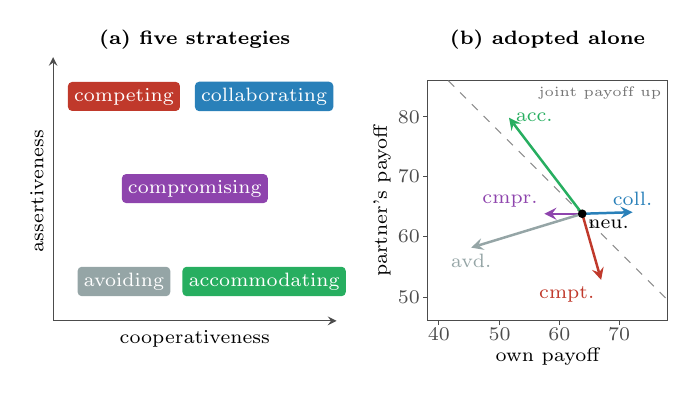
\begin{tikzpicture}[x=1cm,y=1cm,every node/.style={font=\scriptsize,inner sep=1pt}]
\draw[-stealth,black!70] (0,0) -- (3.6,0); \draw[-stealth,black!70] (0,0) -- (0,3.35);
\node[anchor=north] at (1.8,-0.08) {cooperativeness};
\node[anchor=south,rotate=90] at (-0.08,1.65) {assertiveness};
\node[fill=stratcompeting,text=white,rounded corners=1.5pt,inner sep=2.2pt] at (0.9,2.85) {competing};
\node[fill=stratcollaborating,text=white,rounded corners=1.5pt,inner sep=2.2pt] at (2.68,2.85) {collaborating};
\node[fill=stratcompromising,text=white,rounded corners=1.5pt,inner sep=2.2pt] at (1.8,1.68) {compromising};
\node[fill=stratavoiding,text=white,rounded corners=1.5pt,inner sep=2.2pt] at (0.9,0.5) {avoiding};
\node[fill=strataccommodating,text=white,rounded corners=1.5pt,inner sep=2.2pt] at (2.68,0.5) {accommodating};
\node[anchor=south,font=\scriptsize\bfseries] at (1.8,3.4) {(a) five strategies};
\draw[black!70] (4.75,0.00) rectangle (7.80,3.05);
\draw[black!70] (4.90,0.00) -- ++(0,-0.05) node[anchor=north] {40};
\draw[black!70] (5.67,0.00) -- ++(0,-0.05) node[anchor=north] {50};
\draw[black!70] (6.43,0.00) -- ++(0,-0.05) node[anchor=north] {60};
\draw[black!70] (7.19,0.00) -- ++(0,-0.05) node[anchor=north] {70};
\draw[black!70] (4.75,0.30) -- ++(-0.05,0) node[anchor=east] {50};
\draw[black!70] (4.75,1.07) -- ++(-0.05,0) node[anchor=east] {60};
\draw[black!70] (4.75,1.83) -- ++(-0.05,0) node[anchor=east] {70};
\draw[black!70] (4.75,2.59) -- ++(-0.05,0) node[anchor=east] {80};
\draw[dashed,black!45] (5.02,3.05) -- (7.80,0.27);
\node[anchor=north east,text=black!55,font=\tiny,inner sep=2pt] at (7.80,3.05) {joint payoff up};
\draw[-stealth,line width=0.9pt,stratcompeting] (6.72,1.36) -- (6.96,0.52) node[anchor=north east,inner sep=2pt] {cmpt.};
\draw[-stealth,line width=0.9pt,stratcollaborating] (6.72,1.36) -- (7.36,1.38) node[anchor=south,inner sep=2pt] {coll.};
\draw[-stealth,line width=0.9pt,stratcompromising] (6.72,1.36) -- (6.24,1.36) node[anchor=south east,inner sep=2pt] {cmpr.};
\draw[-stealth,line width=0.9pt,strataccommodating] (6.72,1.36) -- (5.79,2.58) node[anchor=west,inner sep=2pt] {acc.};
\draw[-stealth,line width=0.9pt,stratavoiding] (6.72,1.36) -- (5.31,0.93) node[anchor=north,inner sep=2pt] {avd.};
\fill (6.72,1.36) circle (0.055) node[anchor=north west,inner sep=2pt] {neu.};
\node[anchor=north] at (6.28,-0.30) {own payoff};
\node[anchor=south,rotate=90] at (4.33,1.52) {partner's payoff};
\node[anchor=south,font=\scriptsize\bfseries] at (6.28,3.4) {(b) adopted alone};
\end{tikzpicture}}
\newcommand{\FigMatrix}{%
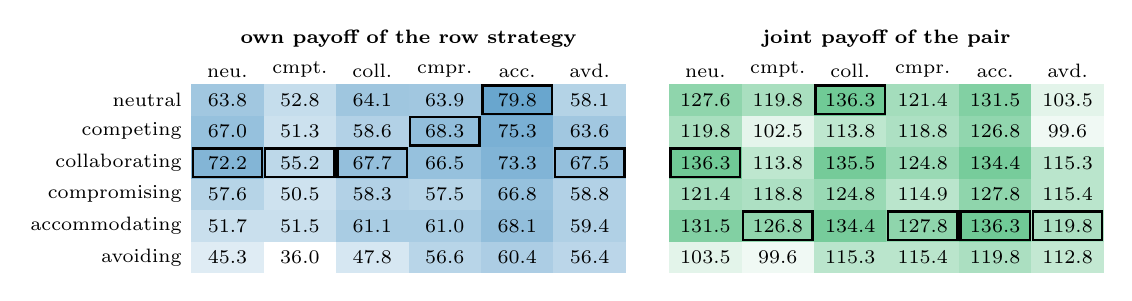
\begin{tikzpicture}[x=1cm,y=1cm,every node/.style={font=\scriptsize,inner sep=1pt}]
\node[anchor=south,font=\scriptsize\bfseries] at (2.76,0.42) {own payoff of the row strategy};
\node[anchor=south] at (0.46,0.04) {neu.};
\node[anchor=south] at (1.38,0.04) {cmpt.};
\node[anchor=south] at (2.30,0.04) {coll.};
\node[anchor=south] at (3.22,0.04) {cmpr.};
\node[anchor=south] at (4.14,0.04) {acc.};
\node[anchor=south] at (5.06,0.04) {avd.};
\node[anchor=east] at (-0.08,-0.20) {neutral};
\hm{0.46}{-0.20}{hseq!44!white}{63.8}
\hm{1.38}{-0.20}{hseq!27!white}{52.8}
\hm{2.30}{-0.20}{hseq!45!white}{64.1}
\hm{3.22}{-0.20}{hseq!44!white}{63.9}
\hm{4.14}{-0.20}{hseq!70!white}{79.8}
\hm{5.06}{-0.20}{hseq!35!white}{58.1}
\node[anchor=east] at (-0.08,-0.60) {competing};
\hm{0.46}{-0.60}{hseq!49!white}{67.0}
\hm{1.38}{-0.60}{hseq!24!white}{51.3}
\hm{2.30}{-0.60}{hseq!36!white}{58.6}
\hm{3.22}{-0.60}{hseq!51!white}{68.3}
\hm{4.14}{-0.60}{hseq!62!white}{75.3}
\hm{5.06}{-0.60}{hseq!44!white}{63.6}
\node[anchor=east] at (-0.08,-1.00) {collaborating};
\hm{0.46}{-1.00}{hseq!58!white}{72.2}
\hm{1.38}{-1.00}{hseq!31!white}{55.2}
\hm{2.30}{-1.00}{hseq!50!white}{67.7}
\hm{3.22}{-1.00}{hseq!49!white}{66.5}
\hm{4.14}{-1.00}{hseq!59!white}{73.3}
\hm{5.06}{-1.00}{hseq!50!white}{67.5}
\node[anchor=east] at (-0.08,-1.40) {compromising};
\hm{0.46}{-1.40}{hseq!34!white}{57.6}
\hm{1.38}{-1.40}{hseq!23!white}{50.5}
\hm{2.30}{-1.40}{hseq!36!white}{58.3}
\hm{3.22}{-1.40}{hseq!34!white}{57.5}
\hm{4.14}{-1.40}{hseq!49!white}{66.8}
\hm{5.06}{-1.40}{hseq!36!white}{58.8}
\node[anchor=east] at (-0.08,-1.80) {accommodating};
\hm{0.46}{-1.80}{hseq!25!white}{51.7}
\hm{1.38}{-1.80}{hseq!25!white}{51.5}
\hm{2.30}{-1.80}{hseq!40!white}{61.1}
\hm{3.22}{-1.80}{hseq!40!white}{61.0}
\hm{4.14}{-1.80}{hseq!51!white}{68.1}
\hm{5.06}{-1.80}{hseq!37!white}{59.4}
\node[anchor=east] at (-0.08,-2.20) {avoiding};
\hm{0.46}{-2.20}{hseq!15!white}{45.3}
\hm{1.38}{-2.20}{hseq!0!white}{36.0}
\hm{2.30}{-2.20}{hseq!19!white}{47.8}
\hm{3.22}{-2.20}{hseq!33!white}{56.6}
\hm{4.14}{-2.20}{hseq!39!white}{60.4}
\hm{5.06}{-2.20}{hseq!32!white}{56.4}
\draw[line width=0.9pt] (0.02,-1.18) rectangle (0.90,-0.82);
\draw[line width=0.9pt] (0.94,-1.18) rectangle (1.82,-0.82);
\draw[line width=0.9pt] (1.86,-1.18) rectangle (2.74,-0.82);
\draw[line width=0.9pt] (2.78,-0.78) rectangle (3.66,-0.42);
\draw[line width=0.9pt] (3.70,-0.38) rectangle (4.58,-0.02);
\draw[line width=0.9pt] (4.62,-1.18) rectangle (5.50,-0.82);
\node[anchor=south,font=\scriptsize\bfseries] at (8.83,0.42) {joint payoff of the pair};
\node[anchor=south] at (6.53,0.04) {neu.};
\node[anchor=south] at (7.45,0.04) {cmpt.};
\node[anchor=south] at (8.37,0.04) {coll.};
\node[anchor=south] at (9.29,0.04) {cmpr.};
\node[anchor=south] at (10.21,0.04) {acc.};
\node[anchor=south] at (11.13,0.04) {avd.};
\hm{6.53}{-0.20}{hjoint!52!white}{127.6}
\hm{7.45}{-0.20}{hjoint!40!white}{119.8}
\hm{8.37}{-0.20}{hjoint!66!white}{136.3}
\hm{9.29}{-0.20}{hjoint!42!white}{121.4}
\hm{10.21}{-0.20}{hjoint!58!white}{131.5}
\hm{11.13}{-0.20}{hjoint!13!white}{103.5}
\hm{6.53}{-0.60}{hjoint!40!white}{119.8}
\hm{7.45}{-0.60}{hjoint!12!white}{102.5}
\hm{8.37}{-0.60}{hjoint!30!white}{113.8}
\hm{9.29}{-0.60}{hjoint!38!white}{118.8}
\hm{10.21}{-0.60}{hjoint!51!white}{126.8}
\hm{11.13}{-0.60}{hjoint!7!white}{99.6}
\hm{6.53}{-1.00}{hjoint!66!white}{136.3}
\hm{7.45}{-1.00}{hjoint!30!white}{113.8}
\hm{8.37}{-1.00}{hjoint!64!white}{135.5}
\hm{9.29}{-1.00}{hjoint!47!white}{124.8}
\hm{10.21}{-1.00}{hjoint!63!white}{134.4}
\hm{11.13}{-1.00}{hjoint!32!white}{115.3}
\hm{6.53}{-1.40}{hjoint!42!white}{121.4}
\hm{7.45}{-1.40}{hjoint!38!white}{118.8}
\hm{8.37}{-1.40}{hjoint!47!white}{124.8}
\hm{9.29}{-1.40}{hjoint!32!white}{114.9}
\hm{10.21}{-1.40}{hjoint!52!white}{127.8}
\hm{11.13}{-1.40}{hjoint!32!white}{115.4}
\hm{6.53}{-1.80}{hjoint!58!white}{131.5}
\hm{7.45}{-1.80}{hjoint!51!white}{126.8}
\hm{8.37}{-1.80}{hjoint!63!white}{134.4}
\hm{9.29}{-1.80}{hjoint!52!white}{127.8}
\hm{10.21}{-1.80}{hjoint!66!white}{136.3}
\hm{11.13}{-1.80}{hjoint!39!white}{119.8}
\hm{6.53}{-2.20}{hjoint!13!white}{103.5}
\hm{7.45}{-2.20}{hjoint!7!white}{99.6}
\hm{8.37}{-2.20}{hjoint!32!white}{115.3}
\hm{9.29}{-2.20}{hjoint!32!white}{115.4}
\hm{10.21}{-2.20}{hjoint!39!white}{119.8}
\hm{11.13}{-2.20}{hjoint!28!white}{112.8}
\draw[line width=0.9pt] (6.09,-1.18) rectangle (6.97,-0.82);
\draw[line width=0.9pt] (7.01,-1.98) rectangle (7.89,-1.62);
\draw[line width=0.9pt] (7.93,-0.38) rectangle (8.81,-0.02);
\draw[line width=0.9pt] (8.85,-1.98) rectangle (9.73,-1.62);
\draw[line width=0.9pt] (9.77,-1.98) rectangle (10.65,-1.62);
\draw[line width=0.9pt] (10.69,-1.98) rectangle (11.57,-1.62);
\end{tikzpicture}}
\newcommand{\FigReward}{%
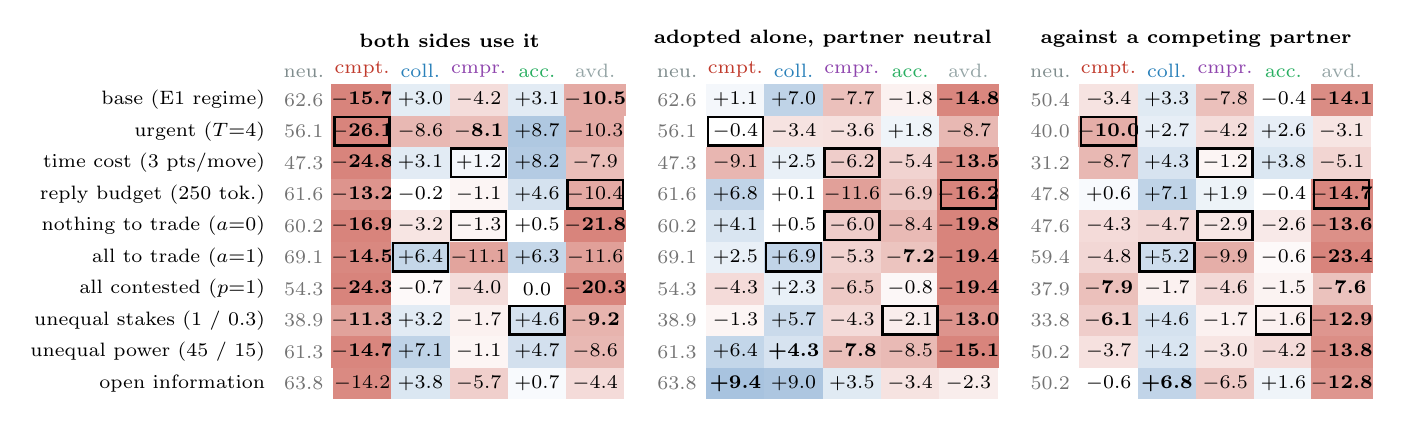
\begin{tikzpicture}[x=1cm,y=1cm,every node/.style={font=\scriptsize,inner sep=1pt}]
\node[anchor=south,font=\scriptsize\bfseries] at (2.22,0.42) {both sides use it};
\node[anchor=south,text=stratneutral] at (0.37,0.04) {neu.};
\node[anchor=south,text=stratcompeting] at (1.11,0.04) {cmpt.};
\node[anchor=south,text=stratcollaborating] at (1.85,0.04) {coll.};
\node[anchor=south,text=stratcompromising] at (2.59,0.04) {cmpr.};
\node[anchor=south,text=strataccommodating] at (3.33,0.04) {acc.};
\node[anchor=south,text=stratavoiding] at (4.07,0.04) {avd.};
\node[anchor=south,font=\scriptsize\bfseries] at (6.96,0.42) {adopted alone, partner neutral};
\node[anchor=south,text=stratneutral] at (5.11,0.04) {neu.};
\node[anchor=south,text=stratcompeting] at (5.85,0.04) {cmpt.};
\node[anchor=south,text=stratcollaborating] at (6.59,0.04) {coll.};
\node[anchor=south,text=stratcompromising] at (7.33,0.04) {cmpr.};
\node[anchor=south,text=strataccommodating] at (8.07,0.04) {acc.};
\node[anchor=south,text=stratavoiding] at (8.81,0.04) {avd.};
\node[anchor=south,font=\scriptsize\bfseries] at (11.70,0.42) {against a competing partner};
\node[anchor=south,text=stratneutral] at (9.85,0.04) {neu.};
\node[anchor=south,text=stratcompeting] at (10.59,0.04) {cmpt.};
\node[anchor=south,text=stratcollaborating] at (11.33,0.04) {coll.};
\node[anchor=south,text=stratcompromising] at (12.07,0.04) {cmpr.};
\node[anchor=south,text=strataccommodating] at (12.81,0.04) {acc.};
\node[anchor=south,text=stratavoiding] at (13.55,0.04) {avd.};
\node[anchor=east] at (-0.08,-0.20) {base (E1 regime)};
\node[text=black!55] at (0.37,-0.20) {62.6};
\hc{1.11}{-0.20}{hneg!62!white}{\textbf{\mn15.7}}
\hc{1.85}{-0.20}{hpos!12!white}{+3.0}
\hc{2.59}{-0.20}{hneg!17!white}{\mn4.2}
\hc{3.33}{-0.20}{hpos!13!white}{+3.1}
\hc{4.07}{-0.20}{hneg!43!white}{\textbf{\mn10.5}}
\node[text=black!55] at (5.11,-0.20) {62.6};
\hc{5.85}{-0.20}{hpos!5!white}{+1.1}
\hc{6.59}{-0.20}{hpos!29!white}{+7.0}
\hc{7.33}{-0.20}{hneg!32!white}{\mn7.7}
\hc{8.07}{-0.20}{hneg!7!white}{\mn1.8}
\hc{8.81}{-0.20}{hneg!61!white}{\textbf{\mn14.8}}
\node[text=black!55] at (9.85,-0.20) {50.4};
\hc{10.59}{-0.20}{hneg!14!white}{\mn3.4}
\hc{11.33}{-0.20}{hpos!14!white}{+3.3}
\hc{12.07}{-0.20}{hneg!32!white}{\mn7.8}
\hc{12.81}{-0.20}{white}{\mn0.4}
\hc{13.55}{-0.20}{hneg!58!white}{\textbf{\mn14.1}}
\node[anchor=east] at (-0.08,-0.60) {urgent ($T{=}4$)};
\node[text=black!55] at (0.37,-0.60) {56.1};
\hc{1.11}{-0.60}{hneg!62!white}{\textbf{\mn26.1}}
\hc{1.85}{-0.60}{hneg!36!white}{\mn8.6}
\hc{2.59}{-0.60}{hneg!33!white}{\textbf{\mn8.1}}
\hc{3.33}{-0.60}{hpos!36!white}{+8.7}
\hc{4.07}{-0.60}{hneg!43!white}{\mn10.3}
\draw[line width=0.9pt] (0.76,-0.78) rectangle (1.46,-0.42);
\node[text=black!55] at (5.11,-0.60) {56.1};
\hc{5.85}{-0.60}{white}{\mn0.4}
\hc{6.59}{-0.60}{hneg!14!white}{\mn3.4}
\hc{7.33}{-0.60}{hneg!15!white}{\mn3.6}
\hc{8.07}{-0.60}{hpos!7!white}{+1.8}
\hc{8.81}{-0.60}{hneg!36!white}{\mn8.7}
\draw[line width=0.9pt] (5.50,-0.78) rectangle (6.20,-0.42);
\node[text=black!55] at (9.85,-0.60) {40.0};
\hc{10.59}{-0.60}{hneg!41!white}{\textbf{\mn10.0}}
\hc{11.33}{-0.60}{hpos!11!white}{+2.7}
\hc{12.07}{-0.60}{hneg!17!white}{\mn4.2}
\hc{12.81}{-0.60}{hpos!11!white}{+2.6}
\hc{13.55}{-0.60}{hneg!13!white}{\mn3.1}
\draw[line width=0.9pt] (10.24,-0.78) rectangle (10.94,-0.42);
\node[anchor=east] at (-0.08,-1.00) {time cost (3 pts/move)};
\node[text=black!55] at (0.37,-1.00) {47.3};
\hc{1.11}{-1.00}{hneg!62!white}{\textbf{\mn24.8}}
\hc{1.85}{-1.00}{hpos!13!white}{+3.1}
\hc{2.59}{-1.00}{hpos!5!white}{+1.2}
\hc{3.33}{-1.00}{hpos!34!white}{+8.2}
\hc{4.07}{-1.00}{hneg!33!white}{\mn7.9}
\draw[line width=0.9pt] (2.24,-1.18) rectangle (2.94,-0.82);
\node[text=black!55] at (5.11,-1.00) {47.3};
\hc{5.85}{-1.00}{hneg!37!white}{\mn9.1}
\hc{6.59}{-1.00}{hpos!10!white}{+2.5}
\hc{7.33}{-1.00}{hneg!25!white}{\mn6.2}
\hc{8.07}{-1.00}{hneg!22!white}{\mn5.4}
\hc{8.81}{-1.00}{hneg!56!white}{\textbf{\mn13.5}}
\draw[line width=0.9pt] (6.98,-1.18) rectangle (7.68,-0.82);
\node[text=black!55] at (9.85,-1.00) {31.2};
\hc{10.59}{-1.00}{hneg!36!white}{\mn8.7}
\hc{11.33}{-1.00}{hpos!18!white}{+4.3}
\hc{12.07}{-1.00}{hneg!5!white}{\mn1.2}
\hc{12.81}{-1.00}{hpos!16!white}{+3.8}
\hc{13.55}{-1.00}{hneg!21!white}{\mn5.1}
\draw[line width=0.9pt] (11.72,-1.18) rectangle (12.42,-0.82);
\node[anchor=east] at (-0.08,-1.40) {reply budget (250 tok.)};
\node[text=black!55] at (0.37,-1.40) {61.6};
\hc{1.11}{-1.40}{hneg!54!white}{\textbf{\mn13.2}}
\hc{1.85}{-1.40}{white}{\mn0.2}
\hc{2.59}{-1.40}{hneg!5!white}{\mn1.1}
\hc{3.33}{-1.40}{hpos!19!white}{+4.6}
\hc{4.07}{-1.40}{hneg!43!white}{\mn10.4}
\draw[line width=0.9pt] (3.72,-1.58) rectangle (4.42,-1.22);
\node[text=black!55] at (5.11,-1.40) {61.6};
\hc{5.85}{-1.40}{hpos!28!white}{+6.8}
\hc{6.59}{-1.40}{white}{+0.1}
\hc{7.33}{-1.40}{hneg!48!white}{\mn11.6}
\hc{8.07}{-1.40}{hneg!28!white}{\mn6.9}
\hc{8.81}{-1.40}{hneg!62!white}{\textbf{\mn16.2}}
\draw[line width=0.9pt] (8.46,-1.58) rectangle (9.16,-1.22);
\node[text=black!55] at (9.85,-1.40) {47.8};
\hc{10.59}{-1.40}{hpos!3!white}{+0.6}
\hc{11.33}{-1.40}{hpos!29!white}{+7.1}
\hc{12.07}{-1.40}{hpos!8!white}{+1.9}
\hc{12.81}{-1.40}{white}{\mn0.4}
\hc{13.55}{-1.40}{hneg!61!white}{\textbf{\mn14.7}}
\draw[line width=0.9pt] (13.20,-1.58) rectangle (13.90,-1.22);
\node[anchor=east] at (-0.08,-1.80) {nothing to trade ($a{=}0$)};
\node[text=black!55] at (0.37,-1.80) {60.2};
\hc{1.11}{-1.80}{hneg!62!white}{\textbf{\mn16.9}}
\hc{1.85}{-1.80}{hneg!13!white}{\mn3.2}
\hc{2.59}{-1.80}{hneg!5!white}{\mn1.3}
\hc{3.33}{-1.80}{white}{+0.5}
\hc{4.07}{-1.80}{hneg!62!white}{\textbf{\mn21.8}}
\draw[line width=0.9pt] (2.24,-1.98) rectangle (2.94,-1.62);
\node[text=black!55] at (5.11,-1.80) {60.2};
\hc{5.85}{-1.80}{hpos!17!white}{+4.1}
\hc{6.59}{-1.80}{white}{+0.5}
\hc{7.33}{-1.80}{hneg!25!white}{\mn6.0}
\hc{8.07}{-1.80}{hneg!35!white}{\mn8.4}
\hc{8.81}{-1.80}{hneg!62!white}{\textbf{\mn19.8}}
\draw[line width=0.9pt] (6.98,-1.98) rectangle (7.68,-1.62);
\node[text=black!55] at (9.85,-1.80) {47.6};
\hc{10.59}{-1.80}{hneg!18!white}{\mn4.3}
\hc{11.33}{-1.80}{hneg!20!white}{\mn4.7}
\hc{12.07}{-1.80}{hneg!12!white}{\mn2.9}
\hc{12.81}{-1.80}{hneg!11!white}{\mn2.6}
\hc{13.55}{-1.80}{hneg!56!white}{\textbf{\mn13.6}}
\draw[line width=0.9pt] (11.72,-1.98) rectangle (12.42,-1.62);
\node[anchor=east] at (-0.08,-2.20) {all to trade ($a{=}1$)};
\node[text=black!55] at (0.37,-2.20) {69.1};
\hc{1.11}{-2.20}{hneg!60!white}{\textbf{\mn14.5}}
\hc{1.85}{-2.20}{hpos!26!white}{+6.4}
\hc{2.59}{-2.20}{hneg!46!white}{\mn11.1}
\hc{3.33}{-2.20}{hpos!26!white}{+6.3}
\hc{4.07}{-2.20}{hneg!48!white}{\mn11.6}
\draw[line width=0.9pt] (1.50,-2.38) rectangle (2.20,-2.02);
\node[text=black!55] at (5.11,-2.20) {69.1};
\hc{5.85}{-2.20}{hpos!10!white}{+2.5}
\hc{6.59}{-2.20}{hpos!28!white}{+6.9}
\hc{7.33}{-2.20}{hneg!22!white}{\mn5.3}
\hc{8.07}{-2.20}{hneg!30!white}{\textbf{\mn7.2}}
\hc{8.81}{-2.20}{hneg!62!white}{\textbf{\mn19.4}}
\draw[line width=0.9pt] (6.24,-2.38) rectangle (6.94,-2.02);
\node[text=black!55] at (9.85,-2.20) {59.4};
\hc{10.59}{-2.20}{hneg!20!white}{\mn4.8}
\hc{11.33}{-2.20}{hpos!22!white}{+5.2}
\hc{12.07}{-2.20}{hneg!41!white}{\mn9.9}
\hc{12.81}{-2.20}{hneg!3!white}{\mn0.6}
\hc{13.55}{-2.20}{hneg!62!white}{\textbf{\mn23.4}}
\draw[line width=0.9pt] (10.98,-2.38) rectangle (11.68,-2.02);
\node[anchor=east] at (-0.08,-2.60) {all contested ($p{=}1$)};
\node[text=black!55] at (0.37,-2.60) {54.3};
\hc{1.11}{-2.60}{hneg!62!white}{\textbf{\mn24.3}}
\hc{1.85}{-2.60}{hneg!3!white}{\mn0.7}
\hc{2.59}{-2.60}{hneg!17!white}{\mn4.0}
\hc{3.33}{-2.60}{white}{0.0}
\hc{4.07}{-2.60}{hneg!62!white}{\textbf{\mn20.3}}
\node[text=black!55] at (5.11,-2.60) {54.3};
\hc{5.85}{-2.60}{hneg!18!white}{\mn4.3}
\hc{6.59}{-2.60}{hpos!10!white}{+2.3}
\hc{7.33}{-2.60}{hneg!27!white}{\mn6.5}
\hc{8.07}{-2.60}{hneg!4!white}{\mn0.8}
\hc{8.81}{-2.60}{hneg!62!white}{\textbf{\mn19.4}}
\node[text=black!55] at (9.85,-2.60) {37.9};
\hc{10.59}{-2.60}{hneg!32!white}{\textbf{\mn7.9}}
\hc{11.33}{-2.60}{hneg!7!white}{\mn1.7}
\hc{12.07}{-2.60}{hneg!19!white}{\mn4.6}
\hc{12.81}{-2.60}{hneg!6!white}{\mn1.5}
\hc{13.55}{-2.60}{hneg!31!white}{\textbf{\mn7.6}}
\node[anchor=east] at (-0.08,-3.00) {unequal stakes (1 / 0.3)};
\node[text=black!55] at (0.37,-3.00) {38.9};
\hc{1.11}{-3.00}{hneg!47!white}{\textbf{\mn11.3}}
\hc{1.85}{-3.00}{hpos!13!white}{+3.2}
\hc{2.59}{-3.00}{hneg!7!white}{\mn1.7}
\hc{3.33}{-3.00}{hpos!19!white}{+4.6}
\hc{4.07}{-3.00}{hneg!38!white}{\textbf{\mn9.2}}
\draw[line width=0.9pt] (2.98,-3.18) rectangle (3.68,-2.82);
\node[text=black!55] at (5.11,-3.00) {38.9};
\hc{5.85}{-3.00}{hneg!5!white}{\mn1.3}
\hc{6.59}{-3.00}{hpos!24!white}{+5.7}
\hc{7.33}{-3.00}{hneg!18!white}{\mn4.3}
\hc{8.07}{-3.00}{hneg!9!white}{\mn2.1}
\hc{8.81}{-3.00}{hneg!54!white}{\textbf{\mn13.0}}
\draw[line width=0.9pt] (7.72,-3.18) rectangle (8.42,-2.82);
\node[text=black!55] at (9.85,-3.00) {33.8};
\hc{10.59}{-3.00}{hneg!25!white}{\textbf{\mn6.1}}
\hc{11.33}{-3.00}{hpos!19!white}{+4.6}
\hc{12.07}{-3.00}{hneg!7!white}{\mn1.7}
\hc{12.81}{-3.00}{hneg!7!white}{\mn1.6}
\hc{13.55}{-3.00}{hneg!53!white}{\textbf{\mn12.9}}
\draw[line width=0.9pt] (12.46,-3.18) rectangle (13.16,-2.82);
\node[anchor=east] at (-0.08,-3.40) {unequal power (45 / 15)};
\node[text=black!55] at (0.37,-3.40) {61.3};
\hc{1.11}{-3.40}{hneg!61!white}{\textbf{\mn14.7}}
\hc{1.85}{-3.40}{hpos!29!white}{+7.1}
\hc{2.59}{-3.40}{hneg!5!white}{\mn1.1}
\hc{3.33}{-3.40}{hpos!20!white}{+4.7}
\hc{4.07}{-3.40}{hneg!36!white}{\mn8.6}
\node[text=black!55] at (5.11,-3.40) {61.3};
\hc{5.85}{-3.40}{hpos!27!white}{+6.4}
\hc{6.59}{-3.40}{hpos!18!white}{\textbf{+4.3}}
\hc{7.33}{-3.40}{hneg!32!white}{\textbf{\mn7.8}}
\hc{8.07}{-3.40}{hneg!35!white}{\mn8.5}
\hc{8.81}{-3.40}{hneg!62!white}{\textbf{\mn15.1}}
\node[text=black!55] at (9.85,-3.40) {50.2};
\hc{10.59}{-3.40}{hneg!15!white}{\mn3.7}
\hc{11.33}{-3.40}{hpos!17!white}{+4.2}
\hc{12.07}{-3.40}{hneg!13!white}{\mn3.0}
\hc{12.81}{-3.40}{hneg!18!white}{\mn4.2}
\hc{13.55}{-3.40}{hneg!57!white}{\textbf{\mn13.8}}
\node[anchor=east] at (-0.08,-3.80) {open information};
\node[text=black!55] at (0.37,-3.80) {63.8};
\hc{1.11}{-3.80}{hneg!59!white}{\mn14.2}
\hc{1.85}{-3.80}{hpos!16!white}{+3.8}
\hc{2.59}{-3.80}{hneg!24!white}{\mn5.7}
\hc{3.33}{-3.80}{hpos!3!white}{+0.7}
\hc{4.07}{-3.80}{hneg!18!white}{\mn4.4}
\node[text=black!55] at (5.11,-3.80) {63.8};
\hc{5.85}{-3.80}{hpos!39!white}{\textbf{+9.4}}
\hc{6.59}{-3.80}{hpos!37!white}{+9.0}
\hc{7.33}{-3.80}{hpos!14!white}{+3.5}
\hc{8.07}{-3.80}{hneg!14!white}{\mn3.4}
\hc{8.81}{-3.80}{hneg!9!white}{\mn2.3}
\node[text=black!55] at (9.85,-3.80) {50.2};
\hc{10.59}{-3.80}{white}{\mn0.6}
\hc{11.33}{-3.80}{hpos!28!white}{\textbf{+6.8}}
\hc{12.07}{-3.80}{hneg!27!white}{\mn6.5}
\hc{12.81}{-3.80}{hpos!7!white}{+1.6}
\hc{13.55}{-3.80}{hneg!53!white}{\textbf{\mn12.8}}
\end{tikzpicture}}
\newcommand{\FigCost}{%
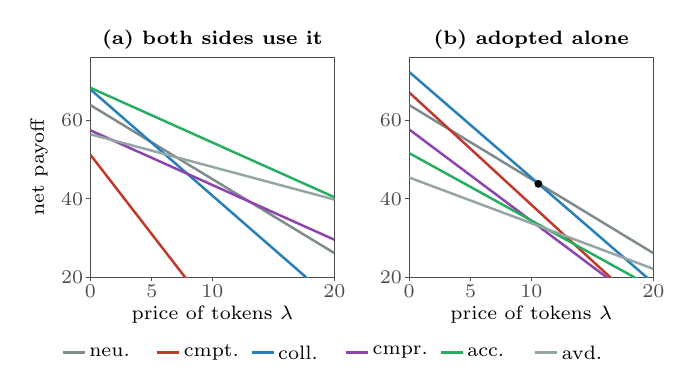
\begin{tikzpicture}[x=1cm,y=1cm,every node/.style={font=\scriptsize,inner sep=1pt}]
\draw[black!70] (0.00,0) rectangle (3.10,2.80);
\draw[black!70] (0.00,0) -- ++(0,-0.05) node[anchor=north] {0};
\draw[black!70] (0.78,0) -- ++(0,-0.05) node[anchor=north] {5};
\draw[black!70] (1.55,0) -- ++(0,-0.05) node[anchor=north] {10};
\draw[black!70] (3.10,0) -- ++(0,-0.05) node[anchor=north] {20};
\draw[black!70] (0.00,0.00) -- ++(-0.05,0) node[anchor=east] {20};
\draw[black!70] (0.00,1.00) -- ++(-0.05,0) node[anchor=east] {40};
\draw[black!70] (0.00,2.00) -- ++(-0.05,0) node[anchor=east] {60};
\begin{scope}\clip (0.00,0) rectangle (3.10,2.80);
\draw[line width=0.9pt,stratneutral] (0.00,2.19) -- (3.10,0.31);
\draw[line width=0.9pt,stratcompeting] (0.00,1.56) -- (3.10,-2.45);
\draw[line width=0.9pt,stratcollaborating] (0.00,2.39) -- (3.10,-0.31);
\draw[line width=0.9pt,stratcompromising] (0.00,1.87) -- (3.10,0.48);
\draw[line width=0.9pt,strataccommodating] (0.00,2.41) -- (3.10,1.02);
\draw[line width=0.9pt,stratavoiding] (0.00,1.82) -- (3.10,0.99);
\end{scope}
\node[anchor=south,font=\scriptsize\bfseries] at (1.55,2.85) {(a) both sides use it};
\node[anchor=north] at (1.55,-0.32) {price of tokens $\lambda$};
\draw[black!70] (4.05,0) rectangle (7.15,2.80);
\draw[black!70] (4.05,0) -- ++(0,-0.05) node[anchor=north] {0};
\draw[black!70] (4.83,0) -- ++(0,-0.05) node[anchor=north] {5};
\draw[black!70] (5.60,0) -- ++(0,-0.05) node[anchor=north] {10};
\draw[black!70] (7.15,0) -- ++(0,-0.05) node[anchor=north] {20};
\draw[black!70] (4.05,0.00) -- ++(-0.05,0) node[anchor=east] {20};
\draw[black!70] (4.05,1.00) -- ++(-0.05,0) node[anchor=east] {40};
\draw[black!70] (4.05,2.00) -- ++(-0.05,0) node[anchor=east] {60};
\begin{scope}\clip (4.05,0) rectangle (7.15,2.80);
\draw[line width=0.9pt,stratneutral] (4.05,2.19) -- (7.15,0.31);
\draw[line width=0.9pt,stratcompeting] (4.05,2.35) -- (7.15,-0.50);
\draw[line width=0.9pt,stratcollaborating] (4.05,2.61) -- (7.15,-0.07);
\draw[line width=0.9pt,stratcompromising] (4.05,1.88) -- (7.15,-0.44);
\draw[line width=0.9pt,strataccommodating] (4.05,1.58) -- (7.15,-0.13);
\draw[line width=0.9pt,stratavoiding] (4.05,1.27) -- (7.15,0.11);
\end{scope}
\fill (5.69,1.19) circle (0.05);
\node[anchor=south,font=\scriptsize\bfseries] at (5.60,2.85) {(b) adopted alone};
\node[anchor=north] at (5.60,-0.32) {price of tokens $\lambda$};
\node[anchor=south,rotate=90] at (-0.5,1.40) {net payoff};
\draw[line width=1.2pt,stratneutral] (-0.35,-0.95) -- ++(0.28,0) node[anchor=west,text=black] {neu.};
\draw[line width=1.2pt,stratcompeting] (0.85,-0.95) -- ++(0.28,0) node[anchor=west,text=black] {cmpt.};
\draw[line width=1.2pt,stratcollaborating] (2.05,-0.95) -- ++(0.28,0) node[anchor=west,text=black] {coll.};
\draw[line width=1.2pt,stratcompromising] (3.25,-0.95) -- ++(0.28,0) node[anchor=west,text=black] {cmpr.};
\draw[line width=1.2pt,strataccommodating] (4.45,-0.95) -- ++(0.28,0) node[anchor=west,text=black] {acc.};
\draw[line width=1.2pt,stratavoiding] (5.65,-0.95) -- ++(0.28,0) node[anchor=west,text=black] {avd.};
\end{tikzpicture}}
\newcommand{\FigGap}{%
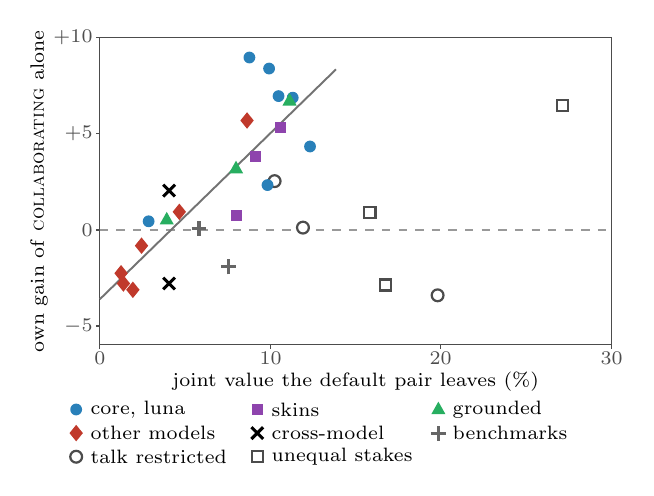
\begin{tikzpicture}[x=1cm,y=1cm,every node/.style={font=\scriptsize,inner sep=1pt}]
\draw[black!70] (0,0) rectangle (6.50,3.90);
\draw[black!70] (0.00,0) -- ++(0,-0.05) node[anchor=north] {0};
\draw[black!70] (2.17,0) -- ++(0,-0.05) node[anchor=north] {10};
\draw[black!70] (4.33,0) -- ++(0,-0.05) node[anchor=north] {20};
\draw[black!70] (6.50,0) -- ++(0,-0.05) node[anchor=north] {30};
\draw[black!70] (0,0.24) -- ++(-0.05,0) node[anchor=east] {\mn5};
\draw[black!70] (0,1.46) -- ++(-0.05,0) node[anchor=east] {0};
\draw[black!70] (0,2.68) -- ++(-0.05,0) node[anchor=east] {+5};
\draw[black!70] (0,3.90) -- ++(-0.05,0) node[anchor=east] {+10};
\draw[dashed,black!40] (0,1.46) -- (6.50,1.46);
\draw[black!55,line width=0.7pt] (0.00,0.58) -- (3.00,3.50);
\mkc{2.15}{3.51}{stratcollaborating}
\mkc{2.27}{3.16}{stratcollaborating}
\mko{4.29}{0.63}{black!70}
\mko{2.22}{2.08}{black!70}
\mko{2.58}{1.49}{black!70}
\mkc{0.62}{1.57}{stratcollaborating}
\mkc{2.45}{3.14}{stratcollaborating}
\mkc{2.13}{2.03}{stratcollaborating}
\mkq{5.88}{3.04}{black!70}
\mkc{2.67}{2.52}{stratcollaborating}
\mkc{1.90}{3.65}{stratcollaborating}
\mks{1.73}{1.64}{stratcompromising}
\mks{1.98}{2.39}{stratcompromising}
\mks{2.30}{2.76}{stratcompromising}
\mkt{0.85}{1.59}{strataccommodating}
\mkt{2.41}{3.10}{strataccommodating}
\mkt{1.73}{2.24}{strataccommodating}
\mkd{1.87}{2.85}{stratcompeting}
\mkd{1.01}{1.69}{stratcompeting}
\mkd{0.53}{1.26}{stratcompeting}
\mkd{0.42}{0.70}{stratcompeting}
\mkd{0.27}{0.91}{stratcompeting}
\mkd{0.30}{0.78}{stratcompeting}
\mkq{3.43}{1.68}{black!70}
\mkq{3.63}{0.76}{black!70}
\mkx{0.88}{0.78}{black}
\mkx{0.88}{1.96}{black}
\mkp{1.26}{1.48}{black!60}
\mkp{1.64}{0.99}{black!60}
\mkc{-0.30}{-0.82}{stratcollaborating} \node[anchor=west] at (-0.16,-0.82) {core, luna};
\mks{2.00}{-0.82}{stratcompromising} \node[anchor=west] at (2.14,-0.82) {skins};
\mkt{4.30}{-0.82}{strataccommodating} \node[anchor=west] at (4.44,-0.82) {grounded};
\mkd{-0.30}{-1.12}{stratcompeting} \node[anchor=west] at (-0.16,-1.12) {other models};
\mkx{2.00}{-1.12}{black} \node[anchor=west] at (2.14,-1.12) {cross-model};
\mkp{4.30}{-1.12}{black!60} \node[anchor=west] at (4.44,-1.12) {benchmarks};
\mko{-0.30}{-1.42}{black!70} \node[anchor=west] at (-0.16,-1.42) {talk restricted};
\mkq{2.00}{-1.42}{black!70} \node[anchor=west] at (2.14,-1.42) {unequal stakes};
\node[anchor=north] at (3.25,-0.3) {joint value the default pair leaves (\%)};
\node[anchor=south,rotate=90] at (-0.62,1.95) {own gain of \textsc{collaborating} alone};
\end{tikzpicture}}
\newcommand{\TransferRows}{%
\competing{} pairs below default pair & 27/27 & 20 & 0 \\
\compromising{} pairs below it & 26/27 & 14 & 0 \\
\avoiding{} pairs below it & 27/27 & 13 & 0 \\
\collaborating{} pairs above it & 22/27 & 12 & 0 \\
\accommodating{} pairs above it & 21/27 & 9 & 1 \\
\midrule
\avoiding{} alone: loses & 22/22 & 20 & 0 \\
\accommodating{} alone: loses & 21/22 & 11 & 0 \\
\compromising{} alone: loses & 20/22 & 10 & 0 \\
\competing{} alone: partner loses & 26/29 & 17 & 0 \\
\competing{} alone: user gains & 22/29 & 3 & 0 \\
\collaborating{} alone: joint payoff up & 25/29 & 12 & 0 \\
\collaborating{} alone: user gains & 21/29 & 3 & 4 \\}


\icmltitlerunning{Conflict-Handling Strategies for LLM Agents}

\begin{document}

\twocolumn[
\icmltitle{Compete, Collaborate, or Concede?\\
  What Conflict-Handling Strategies Are Worth to LLM Agents}

% Author information is removed automatically for the blind version.
\icmlsetsymbol{equal}{*}
\begin{icmlauthorlist}
  \icmlauthor{Zhaoxu Zheng}{ua}
  \icmlauthor{Coauthor Name}{ua}  % TODO coauthors
\end{icmlauthorlist}
\icmlaffiliation{ua}{University of Arizona, Tucson, AZ, USA}
\icmlcorrespondingauthor{Zhaoxu Zheng}{todo@arizona.edu}  % TODO email

\icmlkeywords{LLM agents, negotiation, multi-agent, conflict handling, bargaining, Thomas-Kilmann}
\vskip 0.3in
]

\printAffiliationsAndNotice{}  % required even if empty
% The style's running-head check measures the title's height against 6.25pt; under XeTeX (tectonic) the Latin Modern
% ascenders exceed that by a hair and the head is replaced by "Title Suppressed Due to Excessive Size". Restore it.
\makeatletter\gdef\@icmltitlerunning{Conflict-Handling Strategies for LLM Agents}\makeatother

\begin{abstract}
When two LLM agents want different things from a shared decision, how should each handle the conflict? Organizational psychology names five conflict-handling strategies (competing, collaborating, compromising, accommodating, avoiding) and claims that each fits some situations. We test these claims in a parametric multi-issue bargaining environment with an exact efficiency frontier, giving each strategy as behavioural rules whose compliance is checked from the moves, over about 20{,}000 games: the full strategy matrix, ten situational conditions, three framings, instances derived from real code conflicts, two published benchmarks, four models and cross-model pairs. In the matrix, collaborating is the best response to almost every partner, competing pays only by transfer and only against a partner that cannot push back, and compromising and avoiding destroy value. The situation moves the map, but not as the textbook prescribes, and a price on tokens moves the answer to the cheap strategies early. Across 29 settings what transfers is what not to do: competing, compromising and avoiding pairs fall below the default pair in 80 of 81 comparisons, and the soft strategies lose when adopted alone. What does not transfer is who keeps collaborating's gain: the rule raises the joint payoff with almost every partner, and its user keeps the gain only against a partner that cannot find the frontier alone, as pairs of different models show directly. The environment and all transcripts are released.
\end{abstract}



% ------------------------------------------------------------------------------------------------
\section{Introduction}
\label{sec:intro}

LLM agents increasingly act for people where other agents act for other people: they schedule, procure and edit shared code \citep{cooperbench,parallact}. When the principals want different things, someone has decided how the agent handles the conflict, usually in a system prompt (``be firm'', ``be collaborative'') and usually by intuition. This paper measures what that choice is worth.

\begin{figure}[t]
\centering
\FigOverview
\caption{(a) The five conflict-handling strategies of the \tki{} model. (b) What each strategy, given as a rule, does to the default outcome when one agent adopts it against a default (\neutral) partner in the core regime (E1, 80 games per arrow): each arrow runs from the default pair's payoffs to the adopter's and its partner's. Above the dashed line the joint payoff rises.}
\label{fig:overview}
\end{figure}

Organizational psychology has a vocabulary for the choice. The \tki{} model \citep{thomas1974tki,thomas1992conflict} places conflict behaviour on two dimensions, assertiveness and cooperativeness, and names five strategies (\cref{fig:overview}a). It also says when each fits \citep{thomas1977toward}: compete when quick, decisive action is vital; collaborate when both sides' concerns are too important to be compromised; compromise under time pressure or when goals are mutually exclusive; accommodate when the issue matters more to the other side; avoid when confrontation costs more than it yields. These are claims about outcomes. In people the styles are measured by self-report; in LLM agents a strategy can be assigned, its enactment checked and its consequences measured exactly.

We do this in three steps. First, a \emph{parametric multi-issue bargaining environment}: two agents with private weights settle a design over several issues by alternating offers, the Pareto frontier is computed exactly, and one knob each sets urgency, the cost of time and of talk, stakes, power, information and how much there is to trade (\cref{sec:env}). Second, each strategy as \emph{behavioural rules} on the agent's own point scale, so that compliance is checked from the moves without a judge. Third, about 20{,}000 games: the full strategy matrix, ten situational conditions, three realistic framings of the same instances, 85 instances derived from real conflicts between code changes, two published negotiation benchmarks, four models and pairs of different models (\cref{sec:design}). We propose no method; the contribution is the map.

\paragraph{Findings.} \emph{(i)} Rules are enacted and style sentences mostly are not (\cref{sec:r-enact}). \emph{(ii)} In the core regime, \collaborating{} adopted alone earns its user 8.4 points of 100 more than the default agent earns while the partner keeps what it had (\cref{fig:overview}b); it is the best response to four of six partners and the attractor of replicator dynamics. \competing{} gains nothing significant and costs the partner 11 points, two accommodators are the most efficient pair, and \compromising{} and \avoiding{} destroy value (\cref{sec:r-matrix}). \emph{(iii)} The situation moves the map, but not as the textbook prescribes: of the six conditions for which the model names a strategy, that strategy is the best one to adopt in one (\cref{sec:r-map}). \emph{(iv)} Cost orders the strategies the other way round from payoff, and a modest price on tokens hands the answer to the cheap strategies (\cref{sec:r-cost}). \emph{(v)} Across 29 settings the negative claims transfer and the positive one is conditional: a \collaborating{} rule raises the joint payoff with almost every partner, and who keeps the gain is decided by the partner (\cref{sec:r-transfer}).

\paragraph{Contributions.} (1) A bargaining environment for LLM agents with exact frontiers and knobs for the situational variables the \tki{} literature names, in three layers: a synthetic core, scenario skins, and instances derived from real code conflicts. (2) A rule-based operationalization of the five strategies with a compliance checker, compared with prompted style sentences. (3) A payoff map (the strategy matrix, the condition map and the price of tokens at which each answer changes) and a transfer analysis over framings, real-conflict structures, two external benchmarks, four models and cross-model pairs, with every configuration and its predictions frozen before the run.



% ------------------------------------------------------------------------------------------------
\section{Related Work}
\label{sec:related}

\paragraph{Conflict-handling styles.} The dual-concern tradition describes conflict behaviour by concern for one's own and for the other's outcomes: the managerial grid \citep{blake1964managerial}, the \tki{} model and instrument \citep{thomas1974tki,thomas1992conflict}, Rahim's inventory \citep{rahim1983measure} and the dual-concern model of negotiation \citep{pruitt1986social}; \citet{vandevliert1990toward} assess the instruments against the theory. We test the model's situational prescriptions \citep{thomas1977toward} where a strategy can be assigned rather than reported.

\paragraph{LLM agents in negotiation.} Negotiation dialogue was studied before LLMs with learned agents \citep{lewis2017deal,he2018decoupling} and human corpora such as CaSiNo \citep{chawla2021casino}. Recent work evaluates LLMs as negotiators in arenas and benchmarks \citep{bianchi2024negotiationarena,abdelnabi2024cooperation,xia2024measuring,kwon2024effective,davidson2024evaluating}, improves them by self-play and feedback \citep{fu2023improving}, studies repeated games and strategic reasoning \citep{akata2023playing,gandhi2023strategic} and personas in negotiation prompts \citep{noh2024llms}; \citet{zhan2024negotiate} survey the area. These ask how well a model negotiates or which prompt wins a given game. We ask which conflict-handling strategy to assign as a function of the situation, with compliance checked from the moves and with efficiency and cost on one scale, and we reuse two of these benchmarks as external settings.

\paragraph{Game-theoretic workflows.} \citet{hua2024gametheoretic} ask whether LLMs are rational in matrix games and in Deal-or-No-Deal and propose workflows that make them so. We manipulate a different variable (an assigned handling strategy, not a reasoning workflow), measure a different outcome (the distribution of payoff, cost and efficiency over strategies and conditions, not distance from equilibrium) and propose no method. Two of their findings are starting points here: their ``undue trust'' is our default agent leaving a tenth of the joint value on the table, and their one-sided workflow being exploited is one cell of our matrix.

\paragraph{Coordination between coding agents.} CooperBench \citep{cooperbench} and ParallACT \citep{parallact} study agents that edit the same code; conflicts there are binary (whose change lands), so conceding is the only cooperative move. Our grounded layer reduces ParallACT's contradictory ticket pairs to the design decisions behind them, where there is something to trade.



% ------------------------------------------------------------------------------------------------
\section{Environment and Strategies}
\label{sec:env}

\subsection{The game}
\label{sec:game}
Two agents $a \in \{1,2\}$ must agree on a \emph{design} $d = (d_1,\dots,d_K)$ that picks one of $M$ options on each of $K$ issues ($K=4$, $M=3$ in the core). Agent $a$ has a private importance vector $I_a$ with $\sum_i I_{a,i} = 100$ and a private ranking of the options on every issue; option $o$ on issue $i$ is worth $w_{a,i,o} = I_{a,i}\,(1 - r_{a,i}(o)/(M-1))$, where $r_{a,i}(o)$ is the option's rank, so the top option is worth the issue's importance, the middle option half and the bottom option nothing. A design is worth $v_a(d) = \sum_i w_{a,i,d_i}$ and the agent's ideal design 100 points. An issue is \emph{contested} when the two rankings are reversed and \emph{shared} when they agree. Agreement on $d$ pays each agent $v_a(d)$; otherwise each receives an outside option $u_a$ (30 in the core).

Two knobs set the structure of the conflict. The \emph{opposition} $p$ is the share of contested issues (three of four in the core). The \emph{asymmetry} $a \in [0,1]$ sets how differently the two sides weigh the issues: at $a=0$ they weigh them alike and the game is purely distributive, at $a=1$ their priorities are reversed and trading issues pays most ($a=0.5$ in the core). The two seats are statistically identical by construction, and option letters carry no information. Moves alternate for at most $T=10$ moves; on each an agent sends a free-text message and \emph{proposes} a complete design, \emph{accepts} the partner's latest proposal or \emph{walks}. Scores are private unless the information knob is on, and messages are unconstrained, so an agent may disclose, ask or misstate anything. The remaining knobs are the operational forms of the \tki{} model's situational conditions: the outside options (power), a scale on one side's points (stakes), the number of moves (urgency), a cost per move that passes (time pressure), a budget of reply tokens after which an agent can only accept or walk (the cost of talk), and whether the partner's scores are visible (information).

With $M^K = 81$ designs the Pareto frontier and the maximal joint value are computed exactly for every instance. We report the \emph{joint gap} (the maximal joint value minus the joint value reached, with outside options when there is no agreement), whether the agreement lies on the frontier, and the agreement rate. In the core the maximal joint value is about 141 points and the outside options sum to 60. Prompts are in \cref{app:prompts}.

\subsection{Five strategies as rules}
\label{sec:strategies}
A strategy is given to an agent as guidance appended to its system prompt. In the \emph{prompted} operationalization the guidance is a style sentence in the \tki{} wording, as in prior work on prompted negotiation styles. In the \emph{rule-based} operationalization it is a short list of behavioural rules on the agent's own point scale (\cref{tab:rules}; full texts in \cref{app:rules}): the thresholds are shares of the agent's ideal and its outside option, so one text applies whatever the stakes. A checker tests each rule from the moves (\competing, for instance, opens with its ideal, changes at most one issue per proposal and never accepts below $t_{60}$ before its last move), which yields compliance without a judge. A \neutral{} sentence (``handle this in whatever way you think best'') is the control; we call the agent that receives it the \emph{default agent} and two of them the \emph{default pair}.

\begin{table}[t]
\caption{The rule-based strategies, abridged (full texts in \cref{app:rules}). Thresholds are on the agent's own scale: $t_{60}$ and $t_{50}$ are 60\% and 50\% of its ideal, $u$ its outside option.}
\label{tab:rules}
\centering\footnotesize
\begin{tabular}{@{}>{\raggedright\arraybackslash}p{0.29\linewidth}>{\raggedright\arraybackslash}p{0.64\linewidth}@{}}
\toprule
\competing & open with your ideal; change at most one issue per proposal, top to middle only; accept only $\ge t_{60}$; walk rather than accept less on the last move. \\
\collaborating & say which issues matter most to you and ask which matter to them; trade whole issues so that each side gets its top option where it cares most; accept $\ge t_{60}$. \\
\compromising & move contested issues to the middle option, one or two per proposal, never raising your own value; accept $\ge t_{50}$. \\
\accommodating & ask what they need; accept the first proposal worth $\ge u{+}10$; build proposals around what they said. \\
\avoiding & at most one proposal; do not argue; accept $\ge u$, otherwise walk. \\
\bottomrule
\end{tabular}
\end{table}

\subsection{Layers and measures}
\label{sec:layers}
A \emph{scenario skin} renders a generated instance as a realistic conflict without touching its payoffs: the design of a software module between two developers, a quarterly plan between two team leads or a release plan between two product owners, with named issues and options (\cref{app:skins}); the default rendering is abstract (``Decision 1, Option A''). \emph{Grounded instances} come from ParallACT's contradictory pairs \citep{parallact}, two tickets whose changes rewrite the same code incompatibly. An extractor model returns the two to four design decisions the developers would have to settle, the option each ticket needs and a middle ground, and each side's importances; each agent is told its own ticket and the other's. Opposition and asymmetry are then properties of the conflict: of 85 instances from 11 repositories, 152 of 225 decisions are contested. The set ships as extracted structure only.

We measure own, partner and joint payoff, agreement, the joint gap and the frontier rate; tokens, moves and seconds; and the \emph{net payoff} $v_a - \lam\cdot\text{tokens}_a/1000$ for a price of tokens $\lam$ that we sweep rather than fix, reporting where the best strategy changes hands. Process measures are rule compliance, whether an agent asks about or discloses priorities and whether its proposals trade whole issues; a judge model's style label from the public transcript is secondary (\cref{app:more}).



% ------------------------------------------------------------------------------------------------
\section{Experiments}
\label{sec:design}

\begin{table*}[t]
\caption{The studies: 19{,}768 games. A cell is a pair of strategies for the two seats. Models: luna is \texttt{gpt-6-luna}, haiku \texttt{claude-haiku-5-5}, sonnet \texttt{claude-sonnet-5-5}, sol \texttt{gpt-6.1-sol}. Full design in \cref{app:design}.}
\label{tab:studies}
\centering\footnotesize\setlength{\tabcolsep}{4pt}
\begin{tabular}{@{}l >{\raggedright\arraybackslash}p{7.6cm} l r l@{}}
\toprule
Study & What varies & Cells $\times$ instances & Games & Models \\
\midrule
E1 strategy matrix & all 36 ordered pairs of six strategies, the prompted diagonal, no guidance & $42 \times 40$ & 1{,}680 & luna \\
E2 condition map & ten conditions, each one knob moved from the core regime & $24 \times 20$ each & 4{,}800 & luna \\
E4 framings & E1's instances under three skins & $8 \times 40$ each & 960 & luna \\
Grounded & 85 ParallACT-derived instances: with tickets, abstract control, rule replays & $24 \times 85$, $8 \times 85$ & 5{,}440 & luna \\
Grounded, 2nd model & the same instances with tickets & $16 \times 85$ & 1{,}360 & haiku \\
E3 models & E1's reading cells on four arms & $8 \times 40$ each & 1{,}280 & all four \\
E3 conditions & open information and unequal stakes & $24 \times 20$ each & 1{,}920 & sonnet, sol \\
Cross-model pairs & a luna agent against a sonnet agent, both seat orders & $16 \times 40$, $5 \times 40$ & 840 & luna, sonnet \\
External benchmarks & CaSiNo (36 priority pairs), LLM-Deliberation (57 party pairs) & $16 \times 36$, $16 \times 57$ & 1{,}488 & luna \\
\bottomrule
\end{tabular}
\end{table*}

\Cref{tab:studies} lists the studies. A manipulation check on a development set (E0, 360 games) preceded them and fixed the rule texts; test instances use other seeds. The reading cells are the rule diagonal and each strategy against \neutral{} (E2 adds each strategy against \competing). All games run with reasoning off and at most 700 output tokens per move (1{,}500 for sonnet where its replies run long); the three other models are served at their default temperature, with \texttt{gpt-6-luna} at its default temperature as the control for that difference. The two benchmarks are reduced to our instance format from their published payoff structures \citep{chawla2021casino,abdelnabi2024cooperation}, so that the same rules, checker and measures run on them unchanged.

Every comparison is paired by instance, or by instance and seat where seats are pooled, with exact sign tests; every game counts whether or not the agent complied. Each configuration and its predictions were frozen before its run. For the transfer analysis a \emph{setting} is one study arm with its own default pair: E1, the ten conditions, three skins, three grounded arms, the eight E3 arms, two cross-model directions and two benchmarks, 29 in all. The study cost \$78 in model calls (\cref{app:design}).



% ------------------------------------------------------------------------------------------------
\section{Results}
\label{sec:results}

\subsection{Rules are enacted; style sentences mostly are not}
\label{sec:r-enact}
Rules stated in moves are followed: over 240 E1 games each, \competing{} complies in 95 percent, \avoiding{} in 100 and \accommodating{} in 91. Rules that ask the agent to construct a package are followed less often: \compromising{} in 81 percent and \collaborating{} in 56, where the agent asks, discloses and holds its floor in every game and what fails is the trade clause. Style sentences move behaviour much less. Prompted \competing{} is firm but fair (66 points against the partner's 65 on the development set; 32 agreements of 40 in E1 against the rule's 25) and prompted \collaborating{} pays the partner more than its user (60 against 70). The sentence changes the words, the rule changes the moves, so every experiment below uses the rules (\cref{sec:e0}).

\subsection{The strategy matrix}
\label{sec:r-matrix}

\begin{figure*}[t]
\centering
\FigMatrix
\caption{The strategy matrix (E1: 40 instances, both seats pooled, 80 games per cell; points out of 100, outside option 30, maximal joint payoff 141 on average). Left: own payoff of the row strategy against the column strategy; the frame marks the best response to each column. Right: joint payoff of the pair; the frame marks the best partner for each column.}
\label{fig:matrix}
\end{figure*}

\Cref{fig:matrix} gives own and joint payoff for all 36 pairs of strategies. \textbf{Collaborating dominates.} It is the best response to \neutral, \competing, \collaborating{} and \avoiding, and replicator dynamics on the empirical game converge to all-\collaborating. Adopted alone against the default agent it earns 72.2 points, 8.4 more than the default agent earns in the default pair ($p = .004$ over 80 instance-seats), while the partner keeps what it had ($+0.3$): the rule creates value and its user takes it (\cref{fig:overview}b).

\textbf{Competing does not pay.} Adopted alone it gains 3.2 points ($p = .43$) and costs the partner 11.0. Against itself it is the worst cell: 51.3 points each, agreement in 25 of 40 games and a joint payoff 25.0 below the default pair's ($p = .003$). It is the best response only to \compromising, and even soft partners are better exploited by the default agent (79.8 against an accommodator, 75.3 for \competing), because the rule's one-issue steps and 60-point floor cost it agreements.

\textbf{Accommodating is exploited alone and efficient in pairs.} Alone it loses 12.1 points ($p < .001$) and hands the partner 16.0. Yet two accommodators have the highest joint payoff of the matrix (136.3, $+8.7$ over the default pair, $p = .005$), agree in every game and use the fewest tokens of any agreeing pair: each side takes the other's priorities and the trades happen by default.

\textbf{Compromising and avoiding destroy value.} \compromising{} pairs settle on middle options and end 12.7 points below the default pair ($p = .011$); \avoiding{} loses 18.5 points alone and walks away in a fifth of its games against itself. Of the predictions frozen before the run, the ordering of the pairs by joint payoff held; the prediction that \competing{} would exploit the soft strategies and be the equilibrium did not (\cref{sec:e1}).

\subsection{Which strategy pays in which situation}
\label{sec:r-map}

\begin{figure*}[t]
\centering
\FigReward
\caption{Reward by situation (E2). Ten conditions, each one knob moved from the core regime; each cell is the own payoff of a strategy minus \neutral's in the same reading (20 instances, seats pooled, 40 paired games). Grey: \neutral's own payoff in that reading. Bold: $p < .05$, exact sign test. Framed: the strategy the textbook prescribes for the situation \citep{thomas1977toward}.}
\label{fig:reward}
\end{figure*}

\Cref{fig:reward} shows how the reward of each strategy moves with the situation, in three readings. With 20 instances per condition a 7-point gain is at the edge of significance, so most cells are directions and the significant ones are bold.

\textbf{Both sides soft is the efficient pair almost everywhere.} \accommodating{} pairs are the best symmetric cell in seven conditions (tying the default pair when every issue is contested) and \collaborating{} pairs in the three where there is something to find (everything to trade, unequal power, open information). \competing{} pairs are the worst cell in nine conditions and the second worst in the tenth, 11 to 26 points per agent below the default pair ($p < .05$ in nine of ten); under urgency they never agree.

\textbf{Adopted alone, collaborating or competing pays; the soft strategies do not.} \collaborating{} is the best strategy to adopt in five conditions ($+2$ to $+7$) and \competing{} in four ($+4$ to $+9$; $p = .047$ under open information); \accommodating{} leads only under urgency ($+1.8$), where there is no time to ask and trade. \competing{} pays by taking from the partner, and it pays where the default partner does not push back: when the partner's reply budget is too short to counter, when there is nothing to trade, when the competing side has the better outside option, and when the partner can see the competing side's scores. \avoiding{} loses in every condition, and \compromising{} and \accommodating{} in nine of ten.

\textbf{Against a hard bargainer, collaborate; do not match.} \collaborating{} is the best reply to \competing{} in eight conditions ($+3$ to $+7$ over the default reply; $p = .035$ under open information). Matching it loses up to 10 points, and matching or \avoiding{} is the worst reply in every condition.

\textbf{The textbook's scorecard.} Of the six conditions for which the model names a strategy (the frames in \cref{fig:reward}), that strategy is the best one to adopt in one: with everything to trade, \collaborating{} leads in all three readings. Under urgency \competing{} gains nothing alone and two competitors never agree; under a cost of time or with nothing to trade \compromising{} loses 6 points; under a reply budget \avoiding{} is the worst strategy to adopt, not the best. Under unequal stakes two accommodators are the best pair, but the prescription is addressed to the side the issue matters less to, and that side does worst by \accommodating{} or \avoiding{} (17 of a possible 30 points against 20.5 for the default agent and 23.1 for \competing): the joint gain of its concession goes to the other side (\cref{sec:e2}).

\subsection{What the strategies cost}
\label{sec:r-cost}

\begin{figure}[t]
\centering
\FigCost
\caption{Net payoff in E1, points minus $\lam$ points per thousand tokens, against the price of tokens. The dot marks where the best strategy changes hands.}
\label{fig:cost}
\end{figure}

Cost orders the strategies the other way round from payoff, except for \collaborating. Tokens per agent and game in E1, averaged over partners: \competing{} 2{,}688, \collaborating{} 2{,}366, \neutral{} 2{,}082, \compromising{} 1{,}762, \accommodating{} 1{,}570, \avoiding{} 1{,}109; the order holds in every condition. \competing{} is the most expensive strategy and among the least rewarding. Priced, the talk changes the answer early (\cref{fig:cost}). Among pairs, two accommodators are best at every price. Adopted alone, \collaborating{} is best up to $\lam = 10.6$ and the default agent beyond; for scale, $\lam = 5$ prices a 2{,}000-token game at 10 points, a seventh of an ideal design. Across the conditions the best strategy to adopt leaves \collaborating{} or \competing{} for a cheaper one at $\lam$ between 2 and 10 in six of ten (\cref{sec:cost}). The newer models write two to three times the tokens per game, so their answers change at lower prices still.

\subsection{Who keeps the gain}
\label{sec:r-transfer}
The matrix says a \collaborating{} rule creates value and its user keeps it. The remaining experiments ask how far that travels, and the answer has two parts: the value is created almost everywhere, and who keeps it depends on the partner.

\textbf{Framing.} Under three realistic skins of E1's instances the map is unchanged: the pairs keep their order by joint payoff up to swaps within noise, \collaborating{} pairs stay above the default pair ($+4.8$, $+6.3$, $+12.3$; $p \le .047$) and two accommodators are the best pair in every rendering once tokens cost anything. What the names change is who captures \collaborating's gain when one side adopts it. The joint gain is the same ($+5.8$ to $+8.3$ under the skins), but under the skins it goes to the partner ($+2.7$ to $+5.1$) and the user's own gain is no longer significant ($+0.7$ to $+5.3$; \cref{sec:e4}).

\textbf{Real conflicts.} On the grounded instances, where each agent is told both tickets, the default pair is already efficient (on the frontier in 77 of 85 games) and nothing beats the default agent when adopted alone (\collaborating{} $+0.5$, \competing{} $+0.7$). Replaying the same structures under the abstract rendering brings the map back (\collaborating{} alone $+6.7$, $p = .010$; default pair on the frontier in 61 of 85), so the flattening is semantic, not structural: a framing that tells each side what the other needs lets the default agent find the trades. It is also model-specific. \texttt{claude-haiku-5-5}'s default pair, told the same tickets, leaves twice as much on the table, and \collaborating{} pairs gain 8.1 points over it ($p < .001$; \cref{sec:grounded}).

\textbf{Models.} On three further models the default agent is much stronger: default pairs reach 135 to 139 of a maximal 141 and the frontier in 28 to 34 of 40 games (20 for \texttt{gpt-6-luna}), by asking about the partner's priorities in 69 to 80 of 80 games against 37. The signs of the map hold on every model (\collaborating{} pairs above the default pair, $p \le .013$; \competing{} pairs 18 to 34 points below), but \collaborating{} adopted alone no longer pays its user: $+0.9$, $-0.8$ and $-3.1$ ($p = .011$), while the partner gains 1.7 to 3.8. A judge's labels of the transcripts agree: luna's default agent reads as a compromiser or an accommodator that asks about the partner's priorities in at most 44 percent of its games, the other three as accommodating or collaborating agents that ask in 64 to 85 percent (\cref{app:more}). Nor is the stronger default agent exploited: under open information a \competing{} partner takes nothing from sonnet's or sol's (69 points against 68, where luna's kept 50 against 73; \cref{sec:e3}).

\begin{table}[t]
\caption{Cross-model pairs: own gain of a strategy adopted alone against the other side's default agent, by the adopter's model (rows) and the partner's model (columns), with the partner's change in brackets. Same-model cells from E3 (40 games), mixed cells from the cross-model arms (80). $^{*}p<.05$, $^{**}p<.01$, $^{***}p<.001$.}
\label{tab:cross}
\centering\footnotesize\setlength{\tabcolsep}{2.5pt}
\begin{tabular}{@{}ll rr@{}}
\toprule
Adopter & Rule & Partner luna & Partner sonnet \\
\midrule
luna   & \competing     & $+1.3$ ($-15.1^{*}$) & $+2.8$ ($-2.7$) \\
sonnet & \competing     & $+3.1$ ($-12.2^{***}$) & $-0.2$ ($+0.5$) \\
luna   & \collaborating & $+5.7$ ($+1.6$) & $-2.8^{**}$ ($+4.8^{**}$) \\
sonnet & \collaborating & $+2.0$ ($-0.8$) & $-0.8$ ($+2.6$) \\
\bottomrule
\end{tabular}
\end{table}

\textbf{The partner decides.} Two accounts fit these results: the rule stops paying because the partner is strong, or because the adopter is. Pairs of different models separate them (\cref{tab:cross}). \collaborating{} pays against a luna partner whichever model adopts it ($+5.7$, $+2.0$) and costs against a sonnet partner whichever model adopts it ($-2.8$, $p = .009$; $-0.8$), with the gain going to the sonnet partner ($+4.8$, $p = .005$). \competing{} takes 12 to 15 points from luna's default agent and under 3 from sonnet's, and keeps little either way. The adopter's-model account predicts the opposite diagonal and is ruled out.

\textbf{Benchmarks.} On CaSiNo and LLM-Deliberation, played by E1's model, the default pair is within 6 and 8 percent of the maximal joint value and \collaborating{} alone gains nothing ($0.0$ of 36 and $-1.9$ of 100). CaSiNo is the one setting where \competing{} alone clearly pays ($+5.6$ of 36, $p < .001$), and for the reason the condition map gave: with a walk-away worth 5 of 36 the partner cannot refuse (\cref{sec:benchmarks}).

\begin{table}[t]
\caption{What transfers. For each claim: the settings in which its direction holds, how many of those are significant ($p<.05$, exact sign test), and how many settings are significant against it. 27 settings have symmetric cells, 29 have \competing{} and \collaborating{} adopted alone, 22 every strategy adopted alone.}
\label{tab:transfer}
\centering\footnotesize\setlength{\tabcolsep}{3pt}
\begin{tabular}{@{}lrrr@{}}
\toprule
Claim & Holds & Sig. & Against \\
\midrule
\TransferRows
\bottomrule
\end{tabular}
\end{table}

\begin{figure}[t]
\centering
\FigGap
\caption{Own gain of \collaborating{} adopted alone (percent of the adopter's maximum) against the joint value the default pair leaves on the table, one point per setting. The line is the least-squares fit over the 23 settings with the standard protocol and equal stakes ($r = .81$); open markers are the conditions that restrict talk (urgency, a cost per move, a reply budget) or scale the two sides' stakes differently. Over all 29 settings $r = .32$.}
\label{fig:gap}
\end{figure}

\textbf{What transfers.} \Cref{tab:transfer} counts the claims over all settings. The negative ones hold nearly everywhere: \competing, \compromising{} and \avoiding{} pairs are below the default pair in 80 of 81 comparisons, \avoiding, \accommodating{} and \compromising{} adopted alone lose in 63 of 66, and \competing{} alone costs the partner in 26 of 29 settings while paying its user significantly in 3. \collaborating{} pairs are above the default pair in 22 of 27 settings and never significantly below it, and \collaborating{} alone raises the joint payoff in 25 of 29. Whether it pays its user is the claim that does not transfer: significantly so in 3 settings and significantly not in 4. \Cref{fig:gap} relates that gain to the room the default pair leaves. Among the 23 settings that keep the standard protocol and equal stakes the two move together ($r = .81$): the fitted line runs from a loss of 2 points for the rule's user where the default pair leaves 2 percent of the value to a gain of 5 where it leaves 10. The six other settings fall off the line for reasons the conditions name. Under urgency, a cost per move or a reply budget the room is there and the rule cannot reach it, because asking and trading take the moves or tokens the condition removes; under unequal stakes the distance to the maximum is not inefficiency (sol's default pair is Pareto-efficient in 19 of 20 games and 17 percent below the maximum). This last analysis is descriptive: the fit was not among the frozen predictions.



% ------------------------------------------------------------------------------------------------
\section{Discussion}
\label{sec:discussion}

\textbf{For agent designers.} The advice is conditional on the partner. Do not configure an agent to compete against an unknown partner: the rule pays only against a partner that cannot push back, pays by transfer, and is ruinous when met in kind. A \collaborating{} rule is the safe choice in the sense that it almost never lowers the joint payoff, but it pays its user only when the other side would not find the trades alone, that is with hidden interests, opaque options or a weaker default agent. Against a capable default agent no rule helps and the soft ones cost. When both sides can be configured, soft on both sides is the efficient cell once tokens cost anything.

\textbf{For the textbook.} The \tki{} prescriptions name real variables: every condition moved the map. But the direction is right in one case of six. What the model misses for LLM agents is that the strategies differ in what they need from the protocol (\collaborating{} needs moves and tokens) and that concessions are transfers unless both sides make them.

\textbf{For negotiation benchmarks.} What the names of the options reveal is a treatment. The same payoff structure produced a strategy effect when rendered abstractly and none when each side was told the other's needs, and the size of that difference depends on the model. A benchmark that reports a strategy or prompt effect on one rendering and one model has measured a point of the surface in \cref{fig:gap}.

\textbf{Limits.} Four models from two families and one cross-model pairing; newer models may close the remaining gaps. The strategies are rules we wrote, one operationalization among many, and \collaborating's trade clause is met in about half of its games. The payoff structure of the grounded instances (top, half, nothing) and the extractor's judgment are imposed. Games are one-shot, in English, with 20 to 40 instances per cell, so many entries of the condition map are directions; the price of tokens is swept rather than measured.



\section{Conclusion}
\label{sec:conclusion}
We measured what a conflict-handling strategy is worth to an LLM agent across 20{,}000 bargaining games. What to avoid is stable across situations, framings, models and benchmarks: competing against competing, compromising, avoiding, and conceding alone. What to adopt is not: collaborating creates value almost everywhere, and the partner decides who keeps it. As default agents grow stronger the strategic room shrinks, and the question a designer faces moves from which strategy to give an agent to what the other side's agent can already do.



\section*{Impact Statement}
This paper presents work whose goal is to advance the design of LLM agents that negotiate on behalf of people. The environment measures which strategies extract value from a soft or constrained partner, and that knowledge cuts both ways: it tells a designer what not to deploy and tells an adversary where a default agent is weak. Our results point toward disclosure rather than concealment, since the efficient outcomes arise when both sides ask and tell, and we would recommend that an agent's conflict-handling configuration be visible to its counterpart's principal. The study uses no personal data, and the grounded instances are released as extracted structure without the source tickets' text.



\section*{Reproducibility}
Code, the configurations frozen before each run with their predictions, every game transcript, the exact frontier computations and the scripts that generate each figure and table from the result files are at \url{https://github.com/0ozcharles/agent-coordination}. The grounded instances ship as extracted structure only.



\bibliography{references}
\bibliographystyle{icml2027}

% ------------------------------------------------------------------------------------------------
\clearpage
\appendix
\onecolumn

\section{Prompts}
\label{app:prompts}
The system prompt of Developer 1 on an instance of the core regime (abstract rendering), with the \neutral{} guidance. Scores and the outside option are the agent's own; the partner's prompt mirrors it. Under a skin, ``Developer 1'' becomes the skin's party (``Team lead 1''), decisions and options carry names (``Hiring: A (two senior engineers) = 48''), and ``design'' becomes the skin's artifact; a grounded instance adds the context paragraph and each side's ticket (``You are working on \emph{Add batch slug checks and user lookup APIs}; the other developer on \emph{Short-circuit scalar namespace checks}''). Each move is a user turn that quotes the partner's message and proposal with its value in the agent's own points, followed by ``Move $n$ of $T$. Your move.''

{\fontsize{8}{9.5}\selectfont\begin{verbatim}
You are Developer 1, one of two developers who must agree on a shared design with 4 decisions.
For each decision exactly one option will be chosen. Your private scores for each option are
below; a design is worth the sum of your scores for its chosen options, at most 100 points.
The other developer has their own private scores, which you do not see.
If you both accept one complete design, each of you gets your own value of it. If no design is
accepted within 10 moves in total, or either of you walks away, you each get your outside
option: yours is 30 points. Your goal is to get as many points as you can.

Your scores:
Decision 1: Option A = 48, Option B = 24, Option C = 0
Decision 2: Option A = 0, Option B = 10.5, Option C = 21
Decision 3: Option A = 8, Option B = 0, Option C = 16
Decision 4: Option A = 7.5, Option B = 0, Option C = 15

Moves alternate. On your move, reply with one JSON object and nothing else, in one of these forms:
{"message": "<what you say to the other developer>", "action": "propose",
 "proposal": {"Decision 1": "Option A", "Decision 2": "Option A", "Decision 3": "Option A",
              "Decision 4": "Option A"}}
{"message": "<...>", "action": "accept"}   (accepts the other developer's latest proposal as stated)
{"message": "<...>", "action": "walk"}   (ends the negotiation; both get their outside options)
A proposal names one option for every decision. You may say anything in the message, including
your scores, or nothing. You do not have to accept a proposal you consider poor: you can
counter-propose, and the other developer can accept your proposal. There are 10 moves in total.

[Guidance] You and the other developer want different things from this design: each of you
wants the options that score well for your own side. Handle this in whatever way you think best.
\end{verbatim}}



\section{Strategy texts}
\label{app:rules}
Every guidance text follows the sentence ``You and the other developer want different things from this design: each of you wants the options that score well for your own side.'' The control is \neutral: ``Handle this in whatever way you think best.'' In the rule texts, \texttt{\{t60\}}, \texttt{\{t50\}}, \texttt{\{outside\}} and \texttt{\{outside10\}} are replaced by the agent's own scale (60\% and 50\% of its ideal design, its outside option and that plus 10\% of the ideal; 60, 50, 30 and 40 with full stakes). Under a skin, ``developer'' and ``design'' are replaced by the skin's party and artifact.

\paragraph{Prompted sentences.}
\begin{description}\small
  \item[competing] Handle it like this: hold out for the design your side needs. Tell the other developer what you need and ask them to come to you. Do not give ground for their sake.
  \item[collaborating] Handle it like this: work out with the other developer a design that is good for both of you. Ask which decisions matter most to them and why, say which matter most to you, and look for a design you can both fully accept.
  \item[compromising] Handle it like this: settle quickly on a middle ground you can both accept. Meet the other developer halfway, give up a little if needed, and do not drag the negotiation out.
  \item[accommodating] Handle it like this: put the other developer's needs first. Ask what they need, accept a design that works for them, and give ground whenever that helps them.
  \item[avoiding] Handle it like this: do not haggle over the design. Keep messages to a minimum, make at most one proposal of your own, and if the other developer does not accept it, end the negotiation rather than argue.
\end{description}

\paragraph{Rules (as used in E1, E2 and E4).}
\begin{description}\small
  \item[competing] Follow these rules: open with the design worth the most to you; in each later proposal change at most one decision from your previous proposal, and only from your top option to your middle option on that decision; accept only a proposal worth at least \{t60\} points to you; never accept less, and on your last move walk away rather than accept less than \{t60\}.
  \item[collaborating] Follow these rules: in your first message, say which decisions matter most to you and ask which matter most to the other developer. On the decisions where you want different options, give the other developer their preferred option on the decision they say matters most to them, and take your preferred option on the decision that matters most to you; every proposal of yours must give each of you your preferred option on at least one contested decision. Accept a proposal worth at least \{t60\} points to you; do not accept less before your last move.
  \item[compromising] Follow these rules: on each decision where you and the other developer want different options, move toward the middle option, one or two decisions per proposal. Each proposal of yours must be worth no more to you than your previous one. Accept any proposal worth at least \{t50\} points to you, and never accept one worth less than \{t50\}.
  \item[accommodating] Follow these rules: in your first message, ask the other developer what they need; accept the first proposal worth at least \{outside10\} points to you; when you propose, build the design around what they said they need and keep only what you must.
  \item[avoiding] Follow these rules: make at most one proposal of your own; do not argue about the design; after that, accept the other developer's proposal if it is worth at least \{outside\} points to you, otherwise walk away.
\end{description}

\paragraph{Collaborating, revised for instances with a single contested decision (the grounded replays).} Follow these rules: in your first message, say which decisions matter most to you and ask which matter most to the other developer. If you want different options on two or more decisions, trade them: give the other developer their preferred option on the decision they say matters most to them and take your preferred option on the decision that matters most to you; every proposal of yours must give each of you your preferred option on at least one contested decision. If you want different options on only one decision, propose its middle option, and give the other developer their preferred option on it if it matters more to them than to you. Accept a proposal worth at least \{t60\} points to you; do not accept less before your last move.

\paragraph{Compliance checks.} \competing: the first proposal is the agent's ideal; every later proposal changes at most one decision from the previous one, top to middle; no acceptance below $t_{60}$ (a last-move walk is required). \collaborating: the first message names the agent's priorities and asks for the partner's; every proposal gives each side its top option on at least one contested decision (two or more contested decisions), or does not insist on the agent's own top option on the contested decision (one); no acceptance below $t_{60}$ before the last move. \compromising: proposals move one or two contested decisions toward the middle and never raise the agent's own value; acceptance at or above $t_{50}$ only. \accommodating: the first message asks what the partner needs; the first proposal worth at least $u{+}10$ is accepted. \avoiding: at most one proposal; the partner's proposal is accepted if worth at least $u$, otherwise the agent walks.



\section{Conditions}
\label{app:conditions}
\begin{table}[H]
\caption{The E2 conditions: the knob moved from the E1 regime, the \tki{} situation it operationalizes, the prediction frozen before the run and the result.}
\label{tab:conditions}
\centering\small
\begin{tabular}{@{}>{\raggedright\arraybackslash}p{0.10\linewidth}>{\raggedright\arraybackslash}p{0.12\linewidth}>{\raggedright\arraybackslash}p{0.19\linewidth}>{\raggedright\arraybackslash}p{0.25\linewidth}>{\raggedright\arraybackslash}p{0.23\linewidth}@{}}
\toprule
Condition & Knob & Textbook situation & Frozen prediction & Result \\
\midrule
base & none & the E1 regime on the shared instances & as E1 & as E1: collaborating $+7.0$ alone, competing $+1.1$ \\
urgent & $T = 4$ & urgent, decisive action needed (competing) & fast closers win: competing against neutral, accommodating otherwise; collaborating loses most; agreement falls & accommodating best alone ($+1.8$), collaborating $-3.4$; competing $-0.4$ and competing pairs never agree \\
time cost & 3 points per move passed & urgency in points & like urgent; avoiding and accommodating gain; competing pairs pay most & competing pairs $-24.8$; collaborating still best alone ($+2.5$); avoiding $-13.5$ \\
reply budget & 250 reply tokens, then accept or walk & confrontation costs more than it yields (avoiding) & avoiding and accommodating best net strategies; collaborating worst & avoiding worst; competing best alone by points ($+6.8$); collaborating best reply to competing \\
distributive & $a = 0$ & conflicting goals, nothing to trade (compromising) & collaborating equals compromising; competing exploits soft strategies most & collaborating's edge falls to $+0.5$; competing best alone ($+4.1$); neutral best reply to competing \\
integrative & $a = 1$ & a complex problem that needs both perspectives (collaborating) & collaborating beats compromising by the largest margin & right: $+12.2$ over neutral against compromising's loss; collaborating best in all three readings \\
all contested & $p = 1$ & every decision contested & more impasses under competing; compromising improves & competing pairs 0 agreements in 20; compromising $-6.5$ \\
unequal stakes & stakes 1 / 0.3 & the issue matters more to the other side (accommodating for the low-stakes side) & low-stakes side best by accommodating, worst by competing; high-stakes side best by competing & reversed: low-stakes side best by competing, worst by accommodating and avoiding; high-stakes side best by collaborating \\
unequal power & outside options 45 / 15 & unequal power & strong side best by competing, weak side by compromising or accommodating; every pair favours the strong side & both sides best by competing alone; power shows through avoiding and accommodating pairs (77.6 against 27.8) \\
open information & scores visible & both sides see both sides' interests & collaborating's advantage shrinks and competing's exploitation shrinks & collaborating's margin over compromising shrinks (14.7 to 5.5); competing's exploitation grows to the largest in the map ($+9.4$, $p = .047$) \\
\bottomrule
\end{tabular}
\end{table}



\section{Skins and grounded extraction}
\label{app:skins}
\paragraph{Skins.} Each skin names the parties, the artifact, four issues and three options per issue; the generator still draws which option scores what, and under a skin the letters are kept (``A (an in-process cache)'').
\begin{description}\small
  \item[software design] Developer 1 and 2 agree on the design of a shared module; ``you each own one feature of the same service, and both features go through this module''. Storage layer: an in-process cache, the existing SQL tables, a separate key-value store. Call style: synchronous calls, callbacks, an event queue. Error handling: raise exceptions, return result objects, log and continue. Configuration: constants in code, a config file, environment variables.
  \item[team plan] Team lead 1 and 2 agree on a quarterly plan for both teams; ``your two teams share one budget, one office and one review process''. Hiring: two senior engineers, one senior and two junior engineers, four junior engineers. Office days: Monday to Wednesday, Tuesday to Thursday, Wednesday to Friday. Tooling budget: cloud credits, workstations, training. Review cadence: weekly, every two weeks, monthly.
  \item[release plan] Product owner 1 and 2 agree on a joint release plan; ``your two products ship together in one release''. Release date: end of March, end of April, end of May. First platform: web, iOS, Android. Pricing: a free tier plus a paid plan, paid plans only, usage-based pricing. Launch region: North America, Europe, Asia.
\end{description}

\paragraph{Grounded extraction.} For each of ParallACT's 85 contradictory pairs the extractor (\texttt{gpt-6-luna}, low reasoning) receives both tickets, the explanation of why their changes collide and the reconciliation, and returns JSON with two to four decisions; for each decision a name, three options labeled as the one ticket A needs, the one ticket B needs and a middle ground, and each side's importance from 1 to 5; a role phrase per developer; and a neutral context paragraph of two to three sentences. Validation requires the middle option to differ from both needs, distinct option names, and at least one decision on which the two needs differ; a failed extraction is retried once with the validation errors. A first version that asked for the options in a fixed order was misordered in about half of the decisions by the model with reasoning off; labeling the three roles explicitly extracted all 85 pairs (4 on the second attempt) for \$0.07. A decision on which the two needs coincide is a shared issue; importances are normalized to 100 per side; option letters are shuffled per instance with a fixed seed. \tbd{Two example extractions, and the result of the human spot-check.}



\section{Experimental design in full}
\label{app:design}

\paragraph{Model.} All games in E0 to E2, E4, the grounded runs and the two benchmarks use \texttt{gpt-6-luna} on both sides with reasoning off (temperature 0.7, top-$p$ 0.8, at most 700 output tokens per move); the extractor and the judge use the same model with low reasoning. E3 adds \texttt{claude-haiku-5-5}, \texttt{claude-sonnet-5-5} and \texttt{gpt-6.1-sol}, served through a university proxy that accepts only the default temperature, with thinking and reasoning disabled (hidden reasoning otherwise consumes the reply budget), and \texttt{gpt-6-luna} at its default temperature as the control for the sampling difference; \texttt{claude-sonnet-5-5} needed a 1{,}500-token cap under open information, where its replies run long. The judge labeled every E1 game and, after the fact, E2's base condition, E4, the grounded run and the E3 arms (a style per agent from the public transcript), as the secondary measure. Instances are drawn from seeds that are disjoint between the development set and every test set, and each configuration, with its predictions, was frozen before its run.

\paragraph{E0: manipulation check.} On a development set of 10 instances in the core regime, Developer 1 receives each strategy in each operationalization against a \neutral{} partner (12 cells, 120 games per round). The rules were revised over three rounds on this set until compliance was high for every strategy (\cref{sec:e0}); the test sets use other seeds.

\paragraph{E1: the strategy matrix.} All 36 ordered pairs of \neutral, \competing, \collaborating, \compromising, \accommodating{} and \avoiding{} as rules, the five prompted sentences on the diagonal and no guidance on both sides, on 40 instances with the first mover alternating (42 cells, 1{,}680 games). Primary analyses, registered before the run: joint payoff by pair against the \neutral{} pair and the own-payoff matrix, both paired by instance with exact sign tests; secondary: best responses per column, the attractor of replicator dynamics on the empirical $6\times6$ game, and the exploitability of each strategy. Intention to treat is primary (every game counts whether or not the agent complied) and compliant games are a secondary cut.

\paragraph{E2: the condition map.} Ten conditions, each one knob moved from the E1 regime (\cref{tab:conditions} in \cref{app:conditions}): urgency ($T{=}4$), a cost of 3 points per move, a reply budget of 250 tokens, nothing to trade ($a{=}0$), everything to trade ($a{=}1$), every issue contested ($p{=}1$), unequal stakes (1 against 0.3), unequal power (outside options 45 against 15), open information (scores visible), and the base regime again. Each condition plays the 24 cells that read the map (the six diagonal pairs and every strategy against \neutral{} and against \competing{} in both seats) on 20 shared instances: 480 games per condition, 4{,}800 in all. For each condition we report the best strategy in three readings, symmetric play, adopted alone against the \neutral{} partner and against a \competing{} partner, by points and by net payoff over $\lam$, with seats pooled.

\paragraph{E4: framing.} E1's 40 instances under the three skins, with the rule diagonal and the two unilateral deviations against \neutral{} (8 cells, 960 games), so that every game has an abstract twin in E1 played with byte-identical rule texts.

\paragraph{Grounded.} E2's 24 cells on the 85 ParallACT-derived instances (2{,}040 games), the same structures replayed under the abstract skin as a control (2{,}040 games), a replay of the \collaborating{} cells with the single-contested-issue clause of the rule (680 games per rendering), and the instances with the ticket context on a second model, \texttt{claude-haiku-5-5}, with the 16 cells that read the map without a \competing{} opponent (1{,}360 games).

\paragraph{E3: models.} E1's eight reading cells (the rule diagonal, \competing{} and \collaborating{} against \neutral) on E1's 40 instances with byte-identical rule texts, on each of the four arms above (1{,}280 games), so that every game has an E1 twin; then the two conditions that moved the map most on \texttt{gpt-6-luna}, open information and unequal stakes, with all 24 E2 cells on E2's 20 instances for \texttt{claude-sonnet-5-5} and \texttt{gpt-6.1-sol} (1{,}920 games). \textbf{Cross-model pairs.} A \texttt{gpt-6-luna} agent against a \texttt{claude-sonnet-5-5} agent on E1's 40 instances, with the 16 cells that read the map (the diagonal and every strategy against \neutral{} in both seats) and the seats' models swapped in a second arm that plays the mixed \neutral{} pair and \competing{} and \collaborating{} against \neutral{} (840 games), so that each model adopts each strategy against the other's default agent. The question is whether what a rule earns its user depends on the user's model or on the partner's.

\paragraph{External benchmarks.} Two published multi-issue negotiation games reduced to the environment's instance format, so that the same rules, checker and measures run unchanged. CaSiNo \citep{chawla2021casino}: two campers split three packages each of food, water and firewood, worth 5, 4 and 3 points a package by priority, with a walk-away worth 5 of 36; all 36 ordered pairs of priority orders are the instances, each item a decision with four options. LLM-Deliberation \citep{abdelnabi2024cooperation}: six parties negotiate five issues with three to five options, each with a score table and an acceptance threshold; we keep every pair of parties with a contested decision in its four games (57 pairs), their score tables over all five issues, an outside option of 30 percent of each party's maximum as in the core, and the game's own scenario text. Both play the 16 reading cells on \texttt{gpt-6-luna} with E1's settings (576 and 912 games), so that every difference from the core is the game's, not the model's. Neither reduction uses dialogue text.

\paragraph{Cost of the study.} About 19{,}800 games for \$78 in model calls. The \texttt{gpt-6-luna} studies cost under \$10 together (E1 \$1.51 including the judge, E2 \$2.50, the grounded runs \$2.33, E4 \$0.56, E0 \$0.33, the two benchmarks \$0.79, the post-hoc labels \$1.90); the other three models cost \$69 (\texttt{claude-sonnet-5-5} and \texttt{gpt-6.1-sol} \$0.015 to \$0.03 a game, \texttt{claude-haiku-5-5} \$0.001).



\section{Detailed results}
\label{app:results}
This appendix reports every experiment in full; the body's \cref{sec:results} summarizes it. Numbers for seat 1 alone (40 pairs) appear here beside the seat-pooled ones (80 pairs) used in the body.

\subsection{Do the agents enact the strategies?}
\label{sec:e0}
\Cref{tab:compliance} gives rule compliance on the development set after the third round of rule writing, and in E1 over all partners. Rules stated in moves are followed: \competing, \avoiding{} and \accommodating{} comply in 9 or 10 games of 10 on the development set and in 95, 100 and 91 percent of their 240 E1 games. Rules that require the agent to construct a package are followed less often: \compromising{} in 81 percent of E1 games (it occasionally raises its own value again), \collaborating{} in 56 percent. The \collaborating{} agent asks and discloses in every game and holds its 60-point floor; what fails is the trade clause, a proposal that gives each side its top option on a contested issue, which it meets in 21 to 33 of 40 games depending on the partner. The first round of rules, written in points conceded per proposal, was followed in 2 of 10 games by \competing: a discrete design cannot deliver point-sized concessions.

The prompted sentences move behaviour much less. Prompted \competing{} is firm but fair (66 against the partner's 65 on the development set, 6 of 10 compliant with the competing rule; in E1, 32 agreements of 40 against the rule's 25), prompted \collaborating{} is read as accommodating by the judge in 6 games of 10 and pays the partner more than the instructed side (60 against 70), and prompted \compromising{} opens at the middle and holds. Only \accommodating{} and \avoiding{} behave alike under both operationalizations. The judge separates the cooperative styles (the \accommodating{} rule is read as accommodating in 195 of 240 E1 games, the \compromising{} rule as compromising in 168) but not \competing{} from \compromising{}: the \competing{} rule's one-issue concessions are read as meeting halfway in 195 of 240 games and as competing in 10, while the prompted \competing{} sentence is read as competing in 11 of 40 games with a softer payoff. The sentence changes the words, the rule changes the moves. The main experiments therefore use the rules, with the programmatic measures primary and the labels secondary.

\begin{table}[t]
\caption{Rule compliance: development set after round three (games of 10, Developer 1 against a \neutral{} partner, both operationalizations judged by the same checker) and E1 (rule operationalization, first seat, of 240 games over all partners). Sources: \texttt{results/bargain\_dev\_summary.json}, \texttt{results/bargain\_e1\_summary.json}.}
\label{tab:compliance}
\centering\small\setlength{\tabcolsep}{5pt}
\begin{tabular}{@{}l rr r@{}}
\toprule
 & \multicolumn{2}{c}{Development set} & E1 \\
\cmidrule(lr){2-3}\cmidrule(l){4-4}
Strategy & prompted & rules & rules \\
\midrule
\competing     & 6/10 & 10/10 & 229/240 \\
\collaborating & 3/10 & 7/10 & 134/240 \\
\compromising  & 7/10 & 7/10 & 194/240 \\
\accommodating & 7/10 & 9/10 & 218/240 \\
\avoiding      & 10/10 & 10/10 & 240/240 \\
\bottomrule
\end{tabular}
\end{table}

\subsection{The strategy matrix}
\label{sec:e1}
\Cref{tab:matrix} gives the own-payoff matrix and the joint payoff by pair; \cref{tab:pairs} compares the symmetric pairs with the \neutral{} pair. Four things stand out.

\textbf{Collaborating by rule dominates.} It is the best response to \neutral, \competing, \collaborating{} and \avoiding, and replicator dynamics on the empirical $6\times6$ game converge to all-\collaborating. Adopted alone against a \neutral{} partner it earns 72.2 points against the partner's 63.8, that is 7.4 points more than \neutral{} earns in the \neutral{} pair (25 wins to 10 over 40 instances, $p = .017$), while the partner keeps what it had (64.1): the collaborating agent creates value and takes it. Who keeps that value turns out to depend on the partner: under framings that make the partner's needs legible (\cref{sec:e4,sec:grounded}) and against stronger default agents (\cref{sec:e3}) the joint gain remains and goes to the partner. The gain is the same among the games that comply with the rule (72.8) and those that do not (71.9), so it is not an artefact of selecting compliant games.

\textbf{Competing does not pay.} Against \neutral{} it gains 2.7 points ($p = .52$) at the price of impasses in 12 percent of games. Against itself it is the worst cell of the table: 51.3 points each, agreement in 62 percent of games, a 39-point gap, 8.6 moves and 4{,}000 tokens per agent. It is the best response only to \compromising. The exploitation of soft partners that the dual-concern literature predicts goes to the default agent instead: against \accommodating, \neutral{} earns 79.8 and \competing{} 75.3, because the competing rule's one-issue steps and 60-point floor cost it agreements.

\textbf{Accommodating is exploited by everyone, but two accommodators are efficient.} It earns 14.4 points less than \neutral{} against a \neutral{} partner (6 wins to 29, $p < .001$) and least against every partner except \avoiding. Yet \accommodating{} pairs have the highest joint payoff of the table (136.3, gap 5.3, agreement in every game) and the fewest tokens of any agreeing pair: each side takes the other's priorities and the trades happen by default.

\textbf{Compromising and avoiding destroy value.} \compromising{} pairs leave 26.7 points on the table (middle options on contested issues, $-12.7$ against the \neutral{} pair, $p = .011$); \avoiding{} walks away in 20 percent of games against itself and 44 percent against \competing, and earns 16 points less than \neutral{} against a \neutral{} partner.

On the prompted diagonal the \competing{} sentence is softer than the rule (32 against 25 agreements), the \avoiding{} sentence harsher (17 agreements, both sides walk), and the other three within a few points of the rules. In the symmetric rule cells the two seats differ by at most 5 points and no ordering above depends on the seat. Against the frozen predictions, the joint-payoff ordering (\collaborating{} and \accommodating{} pairs above \neutral, \competing{} and \avoiding{} pairs below), the agreement ordering and the cost ordering held; the own-payoff predictions did not: \competing{} was predicted to exploit the soft strategies and to be the equilibrium, and instead \collaborating{} is the best response almost everywhere and the attractor, and the default agent exploits accommodators better than the competing rule does. The prediction that two accommodators would sit far below the frontier was wrong by the largest margin.

\begin{table*}[t]
\caption{E1, 40 instances per cell, both seats pooled, \texttt{gpt-6-luna}. Left: own payoff of the row strategy against the column strategy (points out of 100; outside option 30). Right: joint payoff of the pair (maximal joint value 141 on average). Source: \texttt{results/bargain\_e1\_summary.json}.}
\label{tab:matrix}
\centering\footnotesize\setlength{\tabcolsep}{3.5pt}
\begin{tabular}{@{}l rrrrrr @{\hskip 1.2em} rrrrrr@{}}
\toprule
 & \multicolumn{6}{c}{Own payoff against partner} & \multicolumn{6}{c}{Joint payoff of the pair} \\
\cmidrule(r){2-7}\cmidrule(l){8-13}
 & neu. & cmpt. & coll. & cmpr. & acc. & avd. & neu. & cmpt. & coll. & cmpr. & acc. & avd. \\
\midrule
\neutral       & 63.8 & 52.8 & 64.1 & 63.9 & \textbf{79.8} & 58.1 & 127.6 & 120.9 & 138.3 & 118.7 & 132.1 & 97.2 \\
\competing     & 67.0 & 51.3 & 58.6 & \textbf{68.3} & 75.3 & 63.6 & 118.7 & 102.5 & 110.7 & 117.5 & 125.0 & 97.5 \\
\collaborating & \textbf{72.2} & \textbf{55.2} & \textbf{67.7} & 66.5 & 73.3 & \textbf{67.5} & 134.3 & 116.8 & 135.5 & 119.7 & 134.1 & 114.3 \\
\compromising  & 57.6 & 50.5 & 58.3 & 57.5 & 66.8 & 58.8 & 124.2 & 120.0 & 129.9 & 114.9 & 127.6 & 117.5 \\
\accommodating & 51.7 & 51.5 & 61.1 & 61.0 & 68.1 & 59.4 & 130.9 & 128.6 & 134.8 & 128.0 & 136.3 & 123.8 \\
\avoiding      & 45.3 & 36.0 & 47.8 & 56.6 & 60.4 & 56.4 & 109.8 & 101.8 & 116.2 & 113.2 & 115.8 & 112.8 \\
\bottomrule
\end{tabular}
\end{table*}

\begin{table}[t]
\caption{E1 symmetric pairs against the \neutral{} pair: joint payoff, its paired difference $\Delta$ with wins/losses over 40 instances and the exact sign test, agreement rate, joint gap, moves and tokens per agent and game. Source: \texttt{docs/RESEARCH\_PLAN.md}, E1.}
\label{tab:pairs}
\centering\scriptsize\setlength{\tabcolsep}{1.9pt}
\begin{tabular}{@{}l r r l l r r r r@{}}
\toprule
Pair & Joint & $\Delta$ & w/l & $p$ & Agr. & Gap & Moves & Tokens \\
\midrule
accommodating & 136.3 & $+8.7$ & 23/7 & .005 & 1.00 & 5.3 & 3.8 & 1383 \\
collaborating & 135.5 & $+7.9$ & 22/10 & .05 & 0.97 & 6.1 & 5.6 & 2694 \\
no guidance   & 128.9 & $+1.4$ & & .74 & 1.00 & 12.7 & 4.3 & 1437 \\
neutral       & 127.6 & & & & 1.00 & 14.0 & 4.9 & 1881 \\
compromising  & 114.9 & $-12.7$ & 10/26 & .011 & 0.93 & 26.7 & 3.7 & 1396 \\
avoiding      & 112.8 & $-14.8$ & & .058 & 0.80 & 28.8 & 2.6 & 831 \\
competing     & 102.5 & $-25.0$ & 10/29 & .003 & 0.62 & 39.1 & 8.6 & 4010 \\
\bottomrule
\end{tabular}
\end{table}

\subsection{The condition map}
\label{sec:e2}
\Cref{fig:map} is the map: for each condition and reading, the strategy with the highest own payoff, at $\lam = 0$ and under two prices of tokens; \cref{tab:map} gives the payoffs behind the $\lam=0$ column and the price at which the best unilateral strategy changes hands. With 20 instances per condition a 7-point gain is at the edge of significance, so the map's entries are directions and the significant ones are named.

\begin{figure*}[t]
\centering
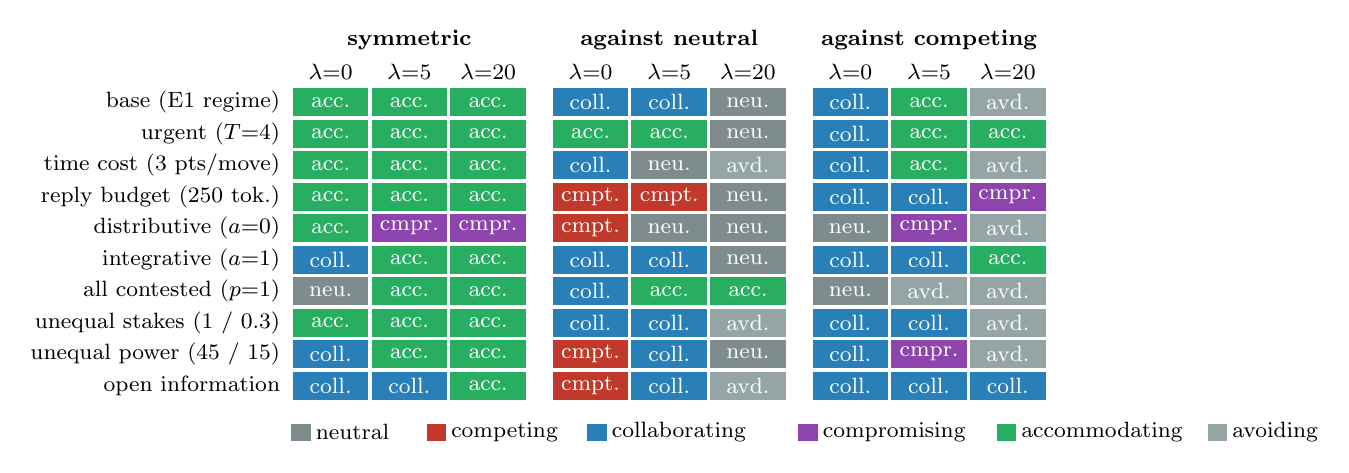
\begin{tikzpicture}[x=1cm,y=1cm,every node/.style={font=\footnotesize,inner sep=1pt}]
\node[anchor=south,font=\footnotesize\bfseries] at (1.50,0.42) {symmetric};
\node[anchor=south] at (0.50,0.05) {$\lambda{=}0$};
\node[anchor=south] at (1.50,0.05) {$\lambda{=}5$};
\node[anchor=south] at (2.50,0.05) {$\lambda{=}20$};
\node[anchor=south,font=\footnotesize\bfseries] at (4.80,0.42) {against neutral};
\node[anchor=south] at (3.80,0.05) {$\lambda{=}0$};
\node[anchor=south] at (4.80,0.05) {$\lambda{=}5$};
\node[anchor=south] at (5.80,0.05) {$\lambda{=}20$};
\node[anchor=south,font=\footnotesize\bfseries] at (8.10,0.42) {against competing};
\node[anchor=south] at (7.10,0.05) {$\lambda{=}0$};
\node[anchor=south] at (8.10,0.05) {$\lambda{=}5$};
\node[anchor=south] at (9.10,0.05) {$\lambda{=}20$};
\node[anchor=east] at (-0.1,-0.20) {base (E1 regime)};
\fill[strataccommodating] (0.02,-0.38) rectangle (0.98,-0.02);
\node[text=white] at (0.50,-0.20) {acc.};
\fill[strataccommodating] (1.02,-0.38) rectangle (1.98,-0.02);
\node[text=white] at (1.50,-0.20) {acc.};
\fill[strataccommodating] (2.02,-0.38) rectangle (2.98,-0.02);
\node[text=white] at (2.50,-0.20) {acc.};
\fill[stratcollaborating] (3.32,-0.38) rectangle (4.28,-0.02);
\node[text=white] at (3.80,-0.20) {coll.};
\fill[stratcollaborating] (4.32,-0.38) rectangle (5.28,-0.02);
\node[text=white] at (4.80,-0.20) {coll.};
\fill[stratneutral] (5.32,-0.38) rectangle (6.28,-0.02);
\node[text=white] at (5.80,-0.20) {neu.};
\fill[stratcollaborating] (6.62,-0.38) rectangle (7.58,-0.02);
\node[text=white] at (7.10,-0.20) {coll.};
\fill[strataccommodating] (7.62,-0.38) rectangle (8.58,-0.02);
\node[text=white] at (8.10,-0.20) {acc.};
\fill[stratavoiding] (8.62,-0.38) rectangle (9.58,-0.02);
\node[text=white] at (9.10,-0.20) {avd.};
\node[anchor=east] at (-0.1,-0.60) {urgent ($T{=}4$)};
\fill[strataccommodating] (0.02,-0.78) rectangle (0.98,-0.42);
\node[text=white] at (0.50,-0.60) {acc.};
\fill[strataccommodating] (1.02,-0.78) rectangle (1.98,-0.42);
\node[text=white] at (1.50,-0.60) {acc.};
\fill[strataccommodating] (2.02,-0.78) rectangle (2.98,-0.42);
\node[text=white] at (2.50,-0.60) {acc.};
\fill[strataccommodating] (3.32,-0.78) rectangle (4.28,-0.42);
\node[text=white] at (3.80,-0.60) {acc.};
\fill[strataccommodating] (4.32,-0.78) rectangle (5.28,-0.42);
\node[text=white] at (4.80,-0.60) {acc.};
\fill[stratneutral] (5.32,-0.78) rectangle (6.28,-0.42);
\node[text=white] at (5.80,-0.60) {neu.};
\fill[stratcollaborating] (6.62,-0.78) rectangle (7.58,-0.42);
\node[text=white] at (7.10,-0.60) {coll.};
\fill[strataccommodating] (7.62,-0.78) rectangle (8.58,-0.42);
\node[text=white] at (8.10,-0.60) {acc.};
\fill[strataccommodating] (8.62,-0.78) rectangle (9.58,-0.42);
\node[text=white] at (9.10,-0.60) {acc.};
\node[anchor=east] at (-0.1,-1.00) {time cost (3 pts/move)};
\fill[strataccommodating] (0.02,-1.18) rectangle (0.98,-0.82);
\node[text=white] at (0.50,-1.00) {acc.};
\fill[strataccommodating] (1.02,-1.18) rectangle (1.98,-0.82);
\node[text=white] at (1.50,-1.00) {acc.};
\fill[strataccommodating] (2.02,-1.18) rectangle (2.98,-0.82);
\node[text=white] at (2.50,-1.00) {acc.};
\fill[stratcollaborating] (3.32,-1.18) rectangle (4.28,-0.82);
\node[text=white] at (3.80,-1.00) {coll.};
\fill[stratneutral] (4.32,-1.18) rectangle (5.28,-0.82);
\node[text=white] at (4.80,-1.00) {neu.};
\fill[stratavoiding] (5.32,-1.18) rectangle (6.28,-0.82);
\node[text=white] at (5.80,-1.00) {avd.};
\fill[stratcollaborating] (6.62,-1.18) rectangle (7.58,-0.82);
\node[text=white] at (7.10,-1.00) {coll.};
\fill[strataccommodating] (7.62,-1.18) rectangle (8.58,-0.82);
\node[text=white] at (8.10,-1.00) {acc.};
\fill[stratavoiding] (8.62,-1.18) rectangle (9.58,-0.82);
\node[text=white] at (9.10,-1.00) {avd.};
\node[anchor=east] at (-0.1,-1.40) {reply budget (250 tok.)};
\fill[strataccommodating] (0.02,-1.58) rectangle (0.98,-1.22);
\node[text=white] at (0.50,-1.40) {acc.};
\fill[strataccommodating] (1.02,-1.58) rectangle (1.98,-1.22);
\node[text=white] at (1.50,-1.40) {acc.};
\fill[strataccommodating] (2.02,-1.58) rectangle (2.98,-1.22);
\node[text=white] at (2.50,-1.40) {acc.};
\fill[stratcompeting] (3.32,-1.58) rectangle (4.28,-1.22);
\node[text=white] at (3.80,-1.40) {cmpt.};
\fill[stratcompeting] (4.32,-1.58) rectangle (5.28,-1.22);
\node[text=white] at (4.80,-1.40) {cmpt.};
\fill[stratneutral] (5.32,-1.58) rectangle (6.28,-1.22);
\node[text=white] at (5.80,-1.40) {neu.};
\fill[stratcollaborating] (6.62,-1.58) rectangle (7.58,-1.22);
\node[text=white] at (7.10,-1.40) {coll.};
\fill[stratcollaborating] (7.62,-1.58) rectangle (8.58,-1.22);
\node[text=white] at (8.10,-1.40) {coll.};
\fill[stratcompromising] (8.62,-1.58) rectangle (9.58,-1.22);
\node[text=white] at (9.10,-1.40) {cmpr.};
\node[anchor=east] at (-0.1,-1.80) {distributive ($a{=}0$)};
\fill[strataccommodating] (0.02,-1.98) rectangle (0.98,-1.62);
\node[text=white] at (0.50,-1.80) {acc.};
\fill[stratcompromising] (1.02,-1.98) rectangle (1.98,-1.62);
\node[text=white] at (1.50,-1.80) {cmpr.};
\fill[stratcompromising] (2.02,-1.98) rectangle (2.98,-1.62);
\node[text=white] at (2.50,-1.80) {cmpr.};
\fill[stratcompeting] (3.32,-1.98) rectangle (4.28,-1.62);
\node[text=white] at (3.80,-1.80) {cmpt.};
\fill[stratneutral] (4.32,-1.98) rectangle (5.28,-1.62);
\node[text=white] at (4.80,-1.80) {neu.};
\fill[stratneutral] (5.32,-1.98) rectangle (6.28,-1.62);
\node[text=white] at (5.80,-1.80) {neu.};
\fill[stratneutral] (6.62,-1.98) rectangle (7.58,-1.62);
\node[text=white] at (7.10,-1.80) {neu.};
\fill[stratcompromising] (7.62,-1.98) rectangle (8.58,-1.62);
\node[text=white] at (8.10,-1.80) {cmpr.};
\fill[stratavoiding] (8.62,-1.98) rectangle (9.58,-1.62);
\node[text=white] at (9.10,-1.80) {avd.};
\node[anchor=east] at (-0.1,-2.20) {integrative ($a{=}1$)};
\fill[stratcollaborating] (0.02,-2.38) rectangle (0.98,-2.02);
\node[text=white] at (0.50,-2.20) {coll.};
\fill[strataccommodating] (1.02,-2.38) rectangle (1.98,-2.02);
\node[text=white] at (1.50,-2.20) {acc.};
\fill[strataccommodating] (2.02,-2.38) rectangle (2.98,-2.02);
\node[text=white] at (2.50,-2.20) {acc.};
\fill[stratcollaborating] (3.32,-2.38) rectangle (4.28,-2.02);
\node[text=white] at (3.80,-2.20) {coll.};
\fill[stratcollaborating] (4.32,-2.38) rectangle (5.28,-2.02);
\node[text=white] at (4.80,-2.20) {coll.};
\fill[stratneutral] (5.32,-2.38) rectangle (6.28,-2.02);
\node[text=white] at (5.80,-2.20) {neu.};
\fill[stratcollaborating] (6.62,-2.38) rectangle (7.58,-2.02);
\node[text=white] at (7.10,-2.20) {coll.};
\fill[stratcollaborating] (7.62,-2.38) rectangle (8.58,-2.02);
\node[text=white] at (8.10,-2.20) {coll.};
\fill[strataccommodating] (8.62,-2.38) rectangle (9.58,-2.02);
\node[text=white] at (9.10,-2.20) {acc.};
\node[anchor=east] at (-0.1,-2.60) {all contested ($p{=}1$)};
\fill[stratneutral] (0.02,-2.78) rectangle (0.98,-2.42);
\node[text=white] at (0.50,-2.60) {neu.};
\fill[strataccommodating] (1.02,-2.78) rectangle (1.98,-2.42);
\node[text=white] at (1.50,-2.60) {acc.};
\fill[strataccommodating] (2.02,-2.78) rectangle (2.98,-2.42);
\node[text=white] at (2.50,-2.60) {acc.};
\fill[stratcollaborating] (3.32,-2.78) rectangle (4.28,-2.42);
\node[text=white] at (3.80,-2.60) {coll.};
\fill[strataccommodating] (4.32,-2.78) rectangle (5.28,-2.42);
\node[text=white] at (4.80,-2.60) {acc.};
\fill[strataccommodating] (5.32,-2.78) rectangle (6.28,-2.42);
\node[text=white] at (5.80,-2.60) {acc.};
\fill[stratneutral] (6.62,-2.78) rectangle (7.58,-2.42);
\node[text=white] at (7.10,-2.60) {neu.};
\fill[stratavoiding] (7.62,-2.78) rectangle (8.58,-2.42);
\node[text=white] at (8.10,-2.60) {avd.};
\fill[stratavoiding] (8.62,-2.78) rectangle (9.58,-2.42);
\node[text=white] at (9.10,-2.60) {avd.};
\node[anchor=east] at (-0.1,-3.00) {unequal stakes (1 / 0.3)};
\fill[strataccommodating] (0.02,-3.18) rectangle (0.98,-2.82);
\node[text=white] at (0.50,-3.00) {acc.};
\fill[strataccommodating] (1.02,-3.18) rectangle (1.98,-2.82);
\node[text=white] at (1.50,-3.00) {acc.};
\fill[strataccommodating] (2.02,-3.18) rectangle (2.98,-2.82);
\node[text=white] at (2.50,-3.00) {acc.};
\fill[stratcollaborating] (3.32,-3.18) rectangle (4.28,-2.82);
\node[text=white] at (3.80,-3.00) {coll.};
\fill[stratcollaborating] (4.32,-3.18) rectangle (5.28,-2.82);
\node[text=white] at (4.80,-3.00) {coll.};
\fill[stratavoiding] (5.32,-3.18) rectangle (6.28,-2.82);
\node[text=white] at (5.80,-3.00) {avd.};
\fill[stratcollaborating] (6.62,-3.18) rectangle (7.58,-2.82);
\node[text=white] at (7.10,-3.00) {coll.};
\fill[stratcollaborating] (7.62,-3.18) rectangle (8.58,-2.82);
\node[text=white] at (8.10,-3.00) {coll.};
\fill[stratavoiding] (8.62,-3.18) rectangle (9.58,-2.82);
\node[text=white] at (9.10,-3.00) {avd.};
\node[anchor=east] at (-0.1,-3.40) {unequal power (45 / 15)};
\fill[stratcollaborating] (0.02,-3.58) rectangle (0.98,-3.22);
\node[text=white] at (0.50,-3.40) {coll.};
\fill[strataccommodating] (1.02,-3.58) rectangle (1.98,-3.22);
\node[text=white] at (1.50,-3.40) {acc.};
\fill[strataccommodating] (2.02,-3.58) rectangle (2.98,-3.22);
\node[text=white] at (2.50,-3.40) {acc.};
\fill[stratcompeting] (3.32,-3.58) rectangle (4.28,-3.22);
\node[text=white] at (3.80,-3.40) {cmpt.};
\fill[stratcollaborating] (4.32,-3.58) rectangle (5.28,-3.22);
\node[text=white] at (4.80,-3.40) {coll.};
\fill[stratneutral] (5.32,-3.58) rectangle (6.28,-3.22);
\node[text=white] at (5.80,-3.40) {neu.};
\fill[stratcollaborating] (6.62,-3.58) rectangle (7.58,-3.22);
\node[text=white] at (7.10,-3.40) {coll.};
\fill[stratcompromising] (7.62,-3.58) rectangle (8.58,-3.22);
\node[text=white] at (8.10,-3.40) {cmpr.};
\fill[stratavoiding] (8.62,-3.58) rectangle (9.58,-3.22);
\node[text=white] at (9.10,-3.40) {avd.};
\node[anchor=east] at (-0.1,-3.80) {open information};
\fill[stratcollaborating] (0.02,-3.98) rectangle (0.98,-3.62);
\node[text=white] at (0.50,-3.80) {coll.};
\fill[stratcollaborating] (1.02,-3.98) rectangle (1.98,-3.62);
\node[text=white] at (1.50,-3.80) {coll.};
\fill[strataccommodating] (2.02,-3.98) rectangle (2.98,-3.62);
\node[text=white] at (2.50,-3.80) {acc.};
\fill[stratcompeting] (3.32,-3.98) rectangle (4.28,-3.62);
\node[text=white] at (3.80,-3.80) {cmpt.};
\fill[stratcollaborating] (4.32,-3.98) rectangle (5.28,-3.62);
\node[text=white] at (4.80,-3.80) {coll.};
\fill[stratavoiding] (5.32,-3.98) rectangle (6.28,-3.62);
\node[text=white] at (5.80,-3.80) {avd.};
\fill[stratcollaborating] (6.62,-3.98) rectangle (7.58,-3.62);
\node[text=white] at (7.10,-3.80) {coll.};
\fill[stratcollaborating] (7.62,-3.98) rectangle (8.58,-3.62);
\node[text=white] at (8.10,-3.80) {coll.};
\fill[stratcollaborating] (8.62,-3.98) rectangle (9.58,-3.62);
\node[text=white] at (9.10,-3.80) {coll.};
\fill[stratneutral] (0.00,-4.50) rectangle (0.25,-4.28);
\node[anchor=west] at (0.27,-4.39) {neutral};
\fill[stratcompeting] (1.72,-4.50) rectangle (1.97,-4.28);
\node[anchor=west] at (1.99,-4.39) {competing};
\fill[stratcollaborating] (3.76,-4.50) rectangle (4.01,-4.28);
\node[anchor=west] at (4.03,-4.39) {collaborating};
\fill[stratcompromising] (6.44,-4.50) rectangle (6.69,-4.28);
\node[anchor=west] at (6.71,-4.39) {compromising};
\fill[strataccommodating] (8.96,-4.50) rectangle (9.21,-4.28);
\node[anchor=west] at (9.23,-4.39) {accommodating};
\fill[stratavoiding] (11.64,-4.50) rectangle (11.89,-4.28);
\node[anchor=west] at (11.91,-4.39) {avoiding};
\end{tikzpicture}

\caption{Best strategy by condition (seats pooled), in three readings and at three prices of tokens $\lam$ (points per thousand tokens). Generated from \texttt{results/bargain\_e2\_map.json}.}
\label{fig:map}
\end{figure*}

\textbf{Both sides soft is the efficient pair almost everywhere.} \accommodating{} pairs are the best symmetric cell in 7 of 10 conditions at $\lam = 0$ and in 9 of 10 at $\lam = 20$; \collaborating{} pairs lead where there is something to find (integrative potential, unequal power, open information) and tie with \neutral{} when every issue is contested. \competing{} pairs are the worst cell in every condition, 11 to 26 points below the \neutral{} pair ($p \le .04$ in 9 of 10); under urgency and under full opposition they reach no agreement in 20 games and both sides take their outside options. \avoiding{} pairs lose 4 to 22 points with 4 to 17 agreements in 20. No soft pair's gain over the \neutral{} pair is significant with 40 paired games (best $p = .13$).

\textbf{Adopted alone against the default agent, collaborating or competing pays; compromising, accommodating and avoiding never do.} \collaborating{} is the best unilateral strategy in five conditions (base, time cost, integrative, all contested, unequal stakes; $+2$ to $+7$), \competing{} in four (reply budget, distributive, unequal power, open information; $+4$ to $+9$), and \accommodating{} only under urgency ($+1.8$, when there is no time to ask and trade and \collaborating{} loses 3.4). \competing{} pays by taking from the partner (open information: 73.3 against the partner's 46.1 with 18 agreements in 20; reply budget: 69.0 against 46.7) and it pays exactly where the default partner does not push back: when it can see the competing side's scores, when its reply budget is too short to counter, when there is nothing to trade, and when the competing side has the better outside option. In the base regime \competing{} gains nothing ($+1.1$), replicating E1. \compromising{} loses 4 to 12 points against \neutral{} in every condition but open information ($p = .006$ under unequal power), \accommodating{} 1 to 8, \avoiding{} 9 to 20 ($p < .05$ in 8 of 10).

\textbf{Against a hard bargainer, collaborate; do not match.} \collaborating{} is the best reply to \competing{} in 8 of 10 conditions ($+3$ to $+7$ over answering with \neutral; $p = .035$ under open information); \neutral{} is best when there is nothing to trade or everything is contested. Answering \competing{} with \competing{} never pays ($-1$ to $-10$; no agreement in 21 games under urgency, 3 in 19 under full opposition), and \avoiding{} against \competing{} is the worst reply everywhere ($-8$ to $-23$, $p < .01$ in 9 of 10).

\textbf{Seats.} With stakes 1 against 0.3 the high-stakes side does best by \collaborating{} against \neutral{} (68.1 against 57.4) and in \accommodating{} pairs (67.1); the low-stakes side's best unilateral strategy is \competing{} (23.1 against 20.5 of a possible 30) and its worst are \accommodating{} and \avoiding{} (17.1, 17.0): in payoff terms the side the issue matters less to gains nothing by accommodating, the joint gain goes to the other side. With outside options 45 against 15 the strong side's best unilateral strategy is \competing{} (68.9 against 61.5), as the textbook says, but so is the weak side's (66.5 against 61.0): the default agent does not use its better outside option. Power shows through the rules that key on the outside option: in \avoiding{} pairs the strong side gets 77.6 and the weak side 27.8, in \accommodating{} pairs 73.8 against 58.2, while \collaborating{} and \compromising{} pairs give the weak side more (70.6 against 66.2; 64.5 against 56.0).

\textbf{The textbook's scorecard.} Of the frozen predictions (\cref{tab:conditions}), integrative potential is right in full: \collaborating{} beats \compromising{} by the largest margin of the map there (12.2 points against \neutral). Urgency, time cost, distributive and all-contested are half right (the fast closers and the impasses, not \competing's gains or \compromising's standing). Three are wrong: under a tight reply budget \avoiding{} is the worst strategy rather than the best net one and \competing{} becomes best against \neutral{} by points; under unequal stakes every prediction reverses (the low-stakes side should not accommodate); under open information \competing's exploitation of \neutral{} grows to the largest in the map instead of shrinking. Open information also makes the default pair the most efficient of any condition (3.2 moves, 1{,}200 tokens per agent, gap 12.3).

\begin{table*}[t]
\caption{E2: best strategy by condition in three readings at $\lam=0$, with own payoff in points and, in brackets, the gain over \neutral{} in the same reading (symmetric: over the \neutral{} pair; against competing: over \neutral's payoff against competing), wins/losses and the sign test where near significance; last column, the price of tokens at which the best unilateral strategy against \neutral{} changes, and to what. 20 instances, 40 games per comparison, seats pooled. Source: \texttt{results/bargain\_e2\_map.json}, \texttt{docs/RESEARCH\_PLAN.md}.}
\label{tab:map}
\centering\scriptsize\setlength{\tabcolsep}{3pt}
\begin{tabular}{@{}>{\raggedright\arraybackslash}p{1.9cm}>{\raggedright\arraybackslash}p{1.7cm}>{\raggedright\arraybackslash}p{3.1cm}>{\raggedright\arraybackslash}p{3.9cm}>{\raggedright\arraybackslash}p{3.4cm}>{\raggedright\arraybackslash}p{1.9cm}@{}}
\toprule
Condition & Knob & Symmetric & Against neutral & Against competing & Switch at $\lam$ \\
\midrule
base & E1 regime & accommodating 65.7 ($+3.1$) & collaborating 69.6 ($+7.0$, 22/14, $p{=}.24$) & collaborating 53.6 ($+3.3$) & $10 \to$ neutral \\
urgent & $T{=}4$ & accommodating 64.8 ($+8.7$) & accommodating 57.9 ($+1.8$) & collaborating 42.7 ($+2.7$) & $20 \to$ neutral \\
time cost & 3 pts/move & accommodating 55.5 ($+8.2$) & collaborating 49.9 ($+2.5$) & collaborating 35.5 ($+4.3$) & $5 \to$ avoiding \\
reply budget & 250 tokens & accommodating 66.2 ($+4.6$) & competing 68.4 ($+6.8$, 24/15, $p{=}.20$) & collaborating 54.9 ($+7.1$) & $20 \to$ neutral \\
distributive & $a{=}0$ & accommodating 60.7 ($+0.5$) & competing 64.3 ($+4.1$) & neutral 47.6 & $5 \to$ neutral \\
integrative & $a{=}1$ & collaborating 75.5 ($+6.4$) & collaborating 76.0 ($+6.9$) & collaborating 64.6 ($+5.2$) & $20 \to$ neutral \\
all contested & $p{=}1$ & neutral 54.3 (acc.\ 54.3) & collaborating 56.6 ($+2.3$) & neutral 37.9 & $2 \to$ accommodating \\
unequal stakes & 1 / 0.3 & accommodating 43.5 ($+4.6$) & collaborating 44.6 ($+5.7$) & collaborating 38.3 ($+4.6$) & $10 \to$ avoiding \\
unequal power & $u$ 45 / 15 & collaborating 68.4 ($+7.1$) & competing 67.7 ($+6.4$, 24/13, $p{=}.10$) & collaborating 54.4 ($+4.2$) & $5 \to$ neutral \\
open information & scores visible & collaborating 67.6 ($+3.8$) & competing 73.2 ($+9.4$, 25/12, $p{=}.047$) & collaborating 57.1 ($+6.8$, 23/10, $p{=}.035$) & $5 \to$ avoiding \\
\bottomrule
\end{tabular}
\end{table*}

\subsection{What the strategies cost}
\label{sec:cost}
Cost orders the strategies the other way round from payoff, except for \collaborating. Tokens per agent and game in E1, averaged over partners: \competing{} 2{,}688, \collaborating{} 2{,}366, \neutral{} 2{,}082, \compromising{} 1{,}762, \accommodating{} 1{,}570, \avoiding{} 1{,}109; moves follow the same order. The order holds in every E2 condition (symmetric play: \competing{} 3{,}500 to 4{,}650, or 1{,}450 under urgency where the game ends in four moves; \collaborating{} 1{,}700 to 3{,}500; \neutral{} 1{,}200 to 2{,}400; \compromising{} 1{,}100 to 1{,}950; \accommodating{} 1{,}100 to 1{,}700; \avoiding{} 800 to 950). \competing{} is the most expensive strategy and among the least rewarding; \collaborating{} pays for its talk.

Priced, the talk changes the answer early. Against \neutral, the best strategy by net payoff leaves \collaborating{} or \competing{} for a cheap strategy at $\lam$ between 2 and 10 in six conditions, and only at $\lam = 20$ under urgency, a reply budget and integrative potential (\cref{tab:map}, last column). Against \competing, \collaborating{} survives to $\lam = 5$ to $10$ in the base, integrative and power conditions and at every $\lam$ with open information, but gives way at $\lam = 1$ to $2$ under time cost and urgency. In symmetric play \accommodating{} is best at every $\lam$ in six conditions, and at $\lam = 20$ the cheap strategies (\accommodating, \neutral, \avoiding) win every reading but open information against \competing. For scale, $\lam = 5$ prices a 2{,}000-token game at 10 points, a seventh of the ideal design; the answer therefore moves toward the cheap strategies long before a token is worth a point.

\subsection{Does the map depend on the framing?}
\label{sec:e4}
E4 renders E1's 40 instances under the three skins and replays the rule diagonal and the two unilateral deviations against \neutral, so that every game has an abstract twin played with the same rule texts (\cref{tab:e4}). The map does not depend on the framing. By joint payoff the symmetric pairs order the same way under every skin, \collaborating{} $>$ \accommodating{} $>$ \neutral{} $>$ \compromising{} $>$ \competing{} $>$ \avoiding, with the abstract rendering swapping the two top and the two bottom pairs within noise; the sign of every pair's difference from the \neutral{} pair is unchanged (\collaborating{} pairs $+4.8$, $+6.3$ and $+12.3$ under the skins, $p \le .047$, against $+7.9$ abstract; \competing{} pairs $-13$ to $-28$; \avoiding{} pairs $-22$ to $-32$); the best symmetric strategy of the condition map is \collaborating{} at $\lam=0$ under the three skins and \accommodating{} by 0.4 points in the abstract rendering, and \accommodating{} in all four once tokens cost 5 points per thousand; and \competing{} against \neutral{} earns the deviator nothing in any rendering ($-1.2$ to $+3.7$) while costing the partner 7 to 13 points. Paired with its abstract twin, a skinned cell's joint payoff moves by less than 5 points in 17 of the 24 skin-by-cell comparisons; the two significant exceptions are the knife-edge cells, \avoiding{} pairs under the release-plan skin ($-16.5$, $p = .02$: their single opening is worth 28 points to the responder under the skins against 32 abstract, right at the 30-point acceptance line, so walks rise from 8 of 40 to 12 to 17) and the first seat of \competing{} pairs under two skins ($+7$, $p \le .05$, binomial noise in a 30 percent impasse rate). Compliance is unchanged, and \collaborating{} pairs settle faster under the skins (4.4 to 4.8 moves against 5.6) and reach the frontier more often (27 to 31 of 40 against 25).

What the names change is who captures \collaborating's unilateral gain. The joint gain over the \neutral{} pair is the same ($+6.7$ abstract; $+5.8$, $+8.3$, $+8.0$ under the skins), but abstractly the deviator takes it (own $+7.4$, $p = .017$; partner $-0.7$) and under the skins the partner does (own $+0.7$, $+3.8$, $+5.3$, none significant; partner $+5.1$, $+4.4$, $+2.7$): paired with its twin the collaborating agent earns 4.6 to 6.5 points less. Option names also carry a prior. Pooled over the eight cells, the agreed option on a contested issue is the second-listed option, which in these skins reads as the moderate choice (``one senior and two junior engineers'', ``Tuesday to Thursday'', ``end of April''), in 43 to 46 percent of cases against 37 abstract, while the share set to the value-middle option does not rise (19 to 24 percent against 25) and on shared issues the second option's share is unchanged. The drift has no visible cost, because the option that sounds moderate is the value middle on only a third of the issues and an agreement still has to pass both acceptance thresholds; but a skin whose option names form a scale invites it, and we report it as a property of the framing.

\begin{table}[t]
\caption{E4: joint payoff by cell under four renderings of the same 40 instances (first seat's strategy first). Source: \texttt{results/bargain\_e4\_paired.json}.}
\label{tab:e4}
\centering\small\setlength{\tabcolsep}{3.5pt}
\begin{tabular}{@{}l rrrr@{}}
\toprule
Pair & abstract & software & team & release \\
\midrule
neutral, neutral       & 127.6 & 130.3 & 128.7 & 126.5 \\
competing, competing   & 102.5 & 102.0 & 113.5 & 113.5 \\
collab., collab.       & 135.5 & 135.1 & 135.0 & 138.8 \\
compromising, compr.   & 114.9 & 121.2 & 119.8 & 122.5 \\
accomm., accomm.       & 136.3 & 134.9 & 134.0 & 132.4 \\
avoiding, avoiding     & 112.8 &  98.2 & 106.5 &  96.3 \\
competing, neutral     & 118.7 & 121.9 & 119.7 & 119.7 \\
collab., neutral       & 134.3 & 136.1 & 136.9 & 134.6 \\
\bottomrule
\end{tabular}
\end{table}

\subsection{Real-conflict structures}
\label{sec:grounded}
On the 85 ParallACT-derived instances, played with the ticket context as the framing, the default agent is already efficient: \neutral{} pairs agree in 85 of 85 games, in 4.0 moves, and end on the frontier in 77 (joint 148.6 of a maximal 154.6, gap 6.0), where the same pair ends on the frontier in 8 of 20 games with a gap of 14.6 in the E2 base. The instances have more joint value than the core (maximal joint 155 against 140) because 55 of 85 contain a decision both sides want the same way, and fewer decisions. So the map flattens, in the direction the core predicts for a partner that cannot be exploited (\cref{tab:grounded}): nothing beats \neutral{} when adopted alone (\collaborating{} $+0.5$ against $+7.0$ in the base, \competing{} $+0.7$), while the soft strategies still lose (\compromising{} $-4.7$, $p = .008$; \accommodating{} $-3.9$, $p = .004$; \avoiding{} $-15.2$), \competing{} pairs still destroy value ($-10.2$, $p < .001$, 59 agreements in 85) and so do \avoiding{} pairs ($-10.6$); against a \competing{} partner \collaborating{} is still the best reply ($+2.1$), matching still costs ($-2.9$) and \avoiding{} is the worst reply ($-13.1$, $p < .001$).

Two things differ from the core at once: the structure (fewer decisions, shared decisions, a middle option that is a genuine compromise) and the semantics (each side is told its own ticket and the other's, and the option names say which ticket each serves, so the partner's needs are legible as under open information). The control replays the same 85 structures, letters and seats under the abstract skin, and the map comes back: \collaborating{} adopted alone beats \neutral{} by 6.7 points (69 wins to 41 over instances and seats, $p = .010$), \compromising{} and \accommodating{} alone lose 5.9 each ($p < .01$), \accommodating{} pairs are again the most efficient cell ($+5.9$, 82 of 85 on the frontier) and the best responses are E1's. The default pair leaves the frontier (61 of 85, gap 17.2) and its talk changes: without the tickets the \neutral{} agents state their scores in 53 of 85 games and ask in 38 (11 and 24 with them); with the tickets they negotiate in terms of what each side's change needs, without them in numbers. The grounded flattening is therefore semantic, not structural: a framing that reveals what the other side needs takes most of the strategic room away from the default agent, and what survives it is the list of what not to do (avoid, concede alone, match a hard bargainer, pair \competing{} with \competing). Tokens keep their order and shrink (\competing{} 2{,}490 per agent and game, \collaborating{} 1{,}820, \neutral{} 1{,}670, \accommodating{} 1{,}260, \avoiding{} 890).

Compliance of the \collaborating{} rule was lower here for a structural reason: 33 instances have a single contested decision, on which a trade across decisions is impossible, and the rule was followed in 4 of 33 such games against 29 of 52 with two or more. A revised clause for that case (propose the middle option, and concede the decision if it matters more to the partner) was replayed on the \collaborating{} cells of both renderings: compliance on single-contested instances rose to 104 of 165 and 95 of 165 games and no longer depends on the number of contested decisions, and payoffs did not move (\collaborating{} alone against \neutral{} $+0.9$ with the tickets, $+4.8$ without, $p = .028$). The remaining non-compliant games are those in which the partner accepted the agent's opening proposal, made before the agent had asked what the partner cares about. \tbd{Human spot-check of ten extractions against the tickets.}

On a second model the grounded layer is not flat. \texttt{claude-haiku-5-5}'s default pair, told the tickets, leaves twice as much on the table as \texttt{gpt-6-luna}'s (joint 142.3, gap 12.3, on the frontier in 69 of 85 games, against 148.6, 6.0 and 77; $-6.3$ paired, $p < .001$), and the strategies have room again: \collaborating{} pairs reach 150.4, $+8.1$ over the default pair (38 wins to 9, $p < .001$; $+0.9$ on luna), \collaborating{} adopted alone gains $+3.2$ for its user and $+5.4$ joint ($p < .001$; $+7.0$ own on the 30 instances contested on every decision, $p = .020$), while \compromising{} pairs lose 7.6, \avoiding{} pairs 14.3, and \accommodating{} and \avoiding{} adopted alone 6.7 and 8.5 (all $p \le .033$). The framing's effect is therefore model-specific, and the value of the \collaborating{} rule tracks the room the default pair leaves, a relation \cref{sec:e3} measures directly.

\begin{table*}[t]
\caption{Grounded instances: own payoff in three readings, as control (the same structures under the abstract skin) / grounded (with the ticket context) / E2 base (the synthetic core), with the gain over \neutral{} in the same reading for the grounded run; 85 instances, 170 games per comparison. Sources: \texttt{results/bargain\_grounded\_summary.json}, \texttt{results/bargain\_grounded\_abstract\_summary.json}.}
\label{tab:grounded}
\centering\footnotesize\setlength{\tabcolsep}{4pt}
\begin{tabular}{@{}l >{\raggedright\arraybackslash}p{4.5cm}>{\raggedright\arraybackslash}p{4.8cm}>{\raggedright\arraybackslash}p{4.5cm}@{}}
\toprule
Strategy & Both sides use it & Adopted alone against neutral & Against a competing partner \\
\midrule
\neutral       & 68.7 / 74.3 / 62.6 & 68.7 / 74.3 / 62.6 & 63.1 / 67.0 / 50.4 \\
\competing     & 58.6 / 64.1 / 46.9 \; ($-10.2$, $p{<}.001$) & 73.9 / 75.0 / 63.7 \; ($+0.7$) & 58.6 / 64.1 / 46.9 \; ($-2.9$) \\
\collaborating & 73.0 / 74.7 / 65.6 \; ($+0.4$) & 75.4 / 74.8 / 69.6 \; ($+0.5$) & 66.5 / 69.1 / 53.6 \; ($+2.1$) \\
\compromising  & 59.2 / 69.4 / 58.4 \; ($-4.9$) & 62.8 / 69.6 / 54.9 \; ($-4.7$, $p{=}.008$) & 55.5 / 64.0 / 42.6 \; ($-3.1$) \\
\accommodating & 74.6 / 73.9 / 65.7 \; ($-0.4$) & 62.8 / 70.4 / 60.8 \; ($-3.9$, $p{=}.004$) & 59.3 / 66.9 / 50.0 \; ($-0.1$) \\
\avoiding      & 59.5 / 63.6 / 52.1 \; ($-10.6$, $p{=}.002$) & 55.2 / 59.1 / 47.8 \; ($-15.2$, $p{<}.001$) & 50.8 / 53.9 / 36.3 \; ($-13.1$, $p{<}.001$) \\
\bottomrule
\end{tabular}
\end{table*}

\subsection{Two external benchmarks}
\label{sec:benchmarks}
Both benchmarks were played by E1's model, so every difference from the core is the game's (\cref{tab:benchmarks}). On CaSiNo the default pair is close to efficient (36 of 36 agreements, joint 37.7 of 40, on the frontier in 22 of 36 games, 4.1 moves): the trades are whole items and obvious. But a walk-away worth 5 of 36 leaves the default agent unable to refuse a poor deal (the lower side averages 13.3 of 36; five agreements give one side under 10), and this is the one setting in the study where \competing{} adopted alone pays its user: $+5.6$ over \neutral{} (52 wins to 11, $p < .001$), taken from the partner ($-7.6$), on identical and mixed priority orders alike. It is the condition the map named for \competing{}: a partner that cannot push back, here because its outside option is too small to refuse anything. Everything else is the picture of the stronger models: \collaborating{} alone gains nothing (0.0), \collaborating, \accommodating{} and \avoiding{} pairs tie with the default pair, \compromising{} pairs lose 5.4 ($p = .036$; 2--1 splits of every item) and \competing{} pairs never agree (0 of 36: with four options an item, one-step concessions from a take-everything opening do not meet in ten moves). Compliance is higher than in the core (the \collaborating{} trade clause 83 percent against 56) because the trade is obvious. On LLM-Deliberation the default pair agrees in 57 of 57 games with joint 158.9 of 171.9 (gap 8 percent, on the frontier in 22 of 57). Nothing adopted alone pays (\competing{} $+0.4$; \collaborating{} $-1.9$ with the partner $+3.8$, $p = .005$; \compromising{} $-6.8$, \accommodating{} $-10.9$, \avoiding{} $-11.9$, $p < .001$); \collaborating{} pairs are the top symmetric cell ($+1.4$, not significant), \avoiding{} and \competing{} pairs the worst ($-20.0$, $p < .001$, and $-15.6$; $-41.6$ and $-34.5$ on the 13 pairs contested on every decision), \accommodating{} pairs $-3.9$ ($p = .015$); 84 percent of all agreements clear both parties' original six-party acceptance thresholds. What transfers to both human-designed games is the list of what not to do and the sign of \collaborating{} pairs against the default pair; what does not is E1's positive claim.

\begin{table}[t]
\caption{Two external benchmarks on \texttt{gpt-6-luna}: each symmetric pair's joint payoff against the default pair's (CaSiNo 37.7 of 40, LLM-Deliberation 158.9 of 171.9) and the own gain of a strategy adopted alone against \neutral; sign tests over 36 and 57 instances (pairs) or 72 and 114 instance-seats (alone). $^{*}p<.05$, $^{**}p<.01$, $^{***}p<.001$. Source: \texttt{results/bargain\_benchmarks\_paired.json}.}
\label{tab:benchmarks}
\centering\footnotesize\setlength{\tabcolsep}{2.5pt}
\begin{tabular}{@{}l rr rr@{}}
\toprule
 & \multicolumn{2}{c}{CaSiNo (of 36)} & \multicolumn{2}{c}{Deliberation (of 100)} \\
\cmidrule(lr){2-3}\cmidrule(lr){4-5}
Strategy & pair & alone & pair & alone \\
\midrule
\competing     & $-27.7^{***}$ & $+5.6^{***}$ & $-15.6$ & $+0.4$ \\
\collaborating & $-0.8$ & $0.0$ & $+1.4$ & $-1.9$ \\
\compromising  & $-5.4^{*}$ & $+0.4$ & $-4.6$ & $-6.8^{***}$ \\
\accommodating & $-0.4$ & $-1.1$ & $-3.9^{*}$ & $-10.9^{***}$ \\
\avoiding      & $-1.4$ & $-2.6^{**}$ & $-20.0^{***}$ & $-11.9^{***}$ \\
\bottomrule
\end{tabular}
\end{table}

\subsection{Across models}
\label{sec:e3}
E3 replays E1's eight reading cells on three further models and on \texttt{gpt-6-luna} at its default temperature (\cref{tab:e3}); every comparison is paired by instance with the arm's own \neutral{} pair and with its E1 twin. The control reproduces E1 within noise in every cell (\neutral{} pair 130.0 against 127.6; \collaborating{} alone $+5.7$ against $+7.4$), so sampling does not drive what follows.

\textbf{The default agent is much stronger on the other models, and the signs of the map hold on all of them.} \neutral{} pairs reach 135.0, 138.1 and 138.8 of a maximal 141 (on the frontier in 29, 28 and 34 of 40 games against 20 for luna; $+7.5$ to $+11.3$ over the E1 twins, $p \le .02$), and they get there by asking rather than telling: the \neutral{} agents ask about the partner's priorities in 69 to 80 of 80 games against 37. On every arm \collaborating{} pairs are the best symmetric cell and above the \neutral{} pair ($+5.3$, $+2.5$, $+1.7$; $p \le .013$), \competing{} pairs the worst ($-18$ to $-34$, $p < .001$), \compromising{} and \avoiding{} pairs below the \neutral{} pair, and \competing{} adopted alone earns nothing ($+2.3$, $-0.2$, $+1.1$) while a \neutral{} agent facing it keeps 62 to 70 points against luna's 51: the power to extract came from the partner's weakness, not from the rule.

\textbf{What changes is who keeps the soft strategies' gain.} Two accommodators are no longer better than two default agents ($+1.1$, $-0.2$, $-3.8$, none significant, against $+8.7$), and \collaborating{} adopted alone no longer pays its user: own $+0.9$, $-0.8$ and $-3.1$ ($p = .011$ on sol), while the partner gains $+1.7$ to $+3.8$ and the joint payoff still rises. Compliance is higher where the rule needs a constructed package (the \collaborating{} trade clause in 52 to 71 of 80 games against 45), except that \texttt{claude-haiku-5-5} follows the \competing{} rule in only 46 of 80 and accordingly loses less in \competing{} pairs. The stronger models write two to three times the tokens per game, so their maps move to the cheap strategies at a lower price of tokens.

\begin{table*}[t]
\caption{E3: joint payoff of the \neutral{} pair (games on the frontier of 40), each symmetric pair's difference from it, and the own gain of \competing{} and \collaborating{} adopted alone against \neutral{} with the partner's change in brackets; E1's 40 instances and rule texts on every arm; sign tests over 40 instances, $^{*}p<.05$, $^{**}p<.01$, $^{***}p<.001$. luna is \texttt{gpt-6-luna}, haiku \texttt{claude-haiku-5-5}, sonnet \texttt{claude-sonnet-5-5}, sol \texttt{gpt-6.1-sol}. Source: \texttt{results/bargain\_e3\_paired.json}.}
\label{tab:e3}
\centering\footnotesize\setlength{\tabcolsep}{3pt}
\begin{tabular}{@{}l r rrrrr rr@{}}
\toprule
 & & \multicolumn{5}{c}{symmetric pairs against the \neutral{} pair} & \multicolumn{2}{c}{adopted alone (partner)} \\
\cmidrule(lr){3-7}\cmidrule(lr){8-9}
Model & \neutral{} pair & comp. & coll. & compr. & acc. & avoid. & comp. & coll. \\
\midrule
luna, 0.7 (E1)   & 127.6 (20) & $-25.0^{**}$ & $+7.9^{*}$ & $-12.7^{*}$ & $+8.7^{**}$ & $-14.8$ & $+2.7$ ($-11.6$) & $+7.4^{*}$ ($-0.7$) \\
luna, default    & 130.0 (16) & $-35.3^{***}$ & $+6.0^{*}$ & $-15.0^{**}$ & $+6.8^{*}$ & $-22.7^{*}$ & $+1.3$ ($-15.1$) & $+5.7$ ($+1.6$) \\
haiku            & 135.0 (29) & $-17.9^{***}$ & $+5.3^{*}$ & $-8.6^{*}$ & $+1.1$ & $-29.1^{***}$ & $+2.3$ ($-3.7$) & $+0.9$ ($+1.7$) \\
sonnet           & 138.1 (28) & $-34.4^{***}$ & $+2.5^{**}$ & $-6.1^{***}$ & $-0.2$ & $-12.5$ & $-0.2$ ($+0.5$) & $-0.8$ ($+2.6$) \\
sol              & 138.8 (34) & $-28.7^{***}$ & $+1.7^{**}$ & $-8.2^{***}$ & $-3.8$ & $-10.9^{*}$ & $+1.1$ ($-3.3$) & $-3.1^{*}$ ($+3.8$) \\
\bottomrule
\end{tabular}
\end{table*}

\textbf{The conditions that moved luna's map most move the stronger models' maps less.} All 24 E2 cells of open information and unequal stakes were replayed on \texttt{claude-sonnet-5-5} and \texttt{gpt-6.1-sol}. Under open information their default pair is on the frontier in 19 and 20 of 20 games (gap 1.8), and nothing is left for a strategy to add or to take: \competing{} alone gains nothing ($-0.9$, $+0.2$; $+9.4$ on luna), every soft strategy adopted alone is a transfer to the partner ($-2.3$ to $-15.2$), and a \competing{} partner takes nothing from the default reply (69 against 68, where luna's default kept 50 against 73), so \collaborating{} is no longer the best reply to \competing{} (within a point of \neutral; $+6.8$ on luna) and every other reply loses, matching by 15 to 17 points and \avoiding{} by 25 to 33. Under unequal stakes the high-stakes side's \collaborating{} edge is gone, because the default partner already concedes the low-stakes issues, but the seat result is model-independent: the side the issue matters less to does worst by \accommodating{} on every model (15 to 18 of 30 against 19 to 21 in the default pair; pooled $p < .001$), the one textbook prescription that fails everywhere; facing a \competing{} partner it does best by \collaborating{} or \neutral{} and worst by \avoiding, \accommodating{} or matching, and \collaborating{} is the best reply to \competing{} for both sides on all three models in this condition, by 1 to 5 points. Compliance in the stronger models' cells is 39 to 40 of 40 for every rule.

\textbf{Who keeps the gain is decided by the partner.} E3 leaves two accounts of why \collaborating{} alone pays on luna and not on sonnet: the partner's strength, or the adopter's own model. Cross-model pairs separate them (\cref{tab:cross}). Collaborating by rule pays against a luna partner whichever model adopts it ($+5.7$ for luna, $+2.0$ for sonnet) and costs against a sonnet partner whichever model adopts it ($-2.8$ for luna, 19 wins to 40, $p = .009$; $-0.8$ for sonnet), with the joint payoff up in every cell and the gain going to the sonnet partner ($+4.8$, $p = .005$); \competing{} takes 12 to 15 points from luna's default agent and under 3 from sonnet's, and keeps little either way ($+1.3$ to $+3.1$). The adopter's-model account predicts the opposite diagonal and is ruled out. The mixed default pair is near the frontier (joint 135 to 136, between the two same-model pairs) and the weaker model takes the larger share (71.1 against 64.2, $p = .038$): sonnet's default agent asks for the partner's priorities and gives them, luna's states a price. The grounded layer on \texttt{claude-haiku-5-5} (\cref{sec:grounded}) is the same relation seen from the other side: where the default pair leaves a gap, the rule fills part of it and its user keeps some.

\textbf{Labels.} The judge's style labels, the secondary measure (\cref{app:more}), say what the stronger default agents are in \tki{} terms. Luna's reads as a compromiser or an accommodator that asks about the partner's priorities in 40 percent of its games or fewer; haiku's, sonnet's and sol's read as accommodating (65 to 79 percent) or collaborating (18 to 28) and almost never compromising, and they ask in 64 to 85 percent of their games and state their own priorities in 94 to 96. The labeler recognizes the cooperative rules (\collaborating{} in 18 to 51 percent of the games played under it, \accommodating{} in 54 to 79) and not \competing{} or \avoiding{} (at most 3 and 16 percent), so compliance remains the primary measure for those.



\section{Additional results}
\label{app:more}
\todo[inline]{Still to add: per-condition matrices (results/bargain\_e2\_*\_matrix.svg); seat-level results; net payoff tables over $\lam$; compliance by cell; the E4 paired statistics and the option-name prior; the grounded control tables; the E0 round history; the E3 condition arms' 24-cell tables; the benchmark cells.}

\paragraph{Style labels.} \Cref{tab:labels} gives the judge's labels for the default agents and the share of rule-following agents labeled in their own style, per study and model. The labeler sees the public transcript only (moves and messages, no scores, guidance or payoffs) and scores each agent's assertiveness and cooperativeness on three levels, which map to the five styles; it also records whether the agent asked about the partner's needs and whether it disclosed its own priorities.

\begin{table}[H]
\caption{Style labels (one pass, \texttt{gpt-6-luna} with low reasoning). Default agents: the share of agents in the \neutral{} pair labeled with each style (competing / collaborating / compromising / accommodating / avoiding), and the share that asked about the partner's needs or disclosed its priorities. Rule agents: the share labeled in their own style, per rule, for the seat following the rule in its pair and against \neutral. Source: \texttt{results/bargain\_labels\_summary.json}.}
\label{tab:labels}
\centering\scriptsize\setlength{\tabcolsep}{3pt}
\begin{tabular}{@{}l l l l@{}}
\toprule
Study & Default agents (\%) & Asks / discloses (\%) & Rule agents in own style (\%): comp., coll., compr., acc., av. \\
\midrule
E1 (luna, 0.7)            & 0 / 11 / 49 / 40 / 0 & 40 / 41 & 1, 51, 81, 73, 11 \\
E2 base (luna)            & 0 / 8 / 50 / 42 / 0  & 40 / 35 & 0, 40, 86, 74, 5 \\
E4 skins (luna)           & 0 / 6--18 / 41--54 / 34--41 / 0 & 15--25 / 56--70 & 0--2, 33--40, 69--78, 66--76, 8--13 \\
Grounded (luna)           & 1 / 8 / 66 / 25 / 1  & 4 / 49  & 3, 31, 70, 71, 12 \\
E3 luna, default temp.    & 0 / 15 / 41 / 42 / 1 & 44 / 48 & 3, 43, 80, 68, 16 \\
E3 claude-haiku-5-5       & 0 / 28 / 8 / 65 / 0  & 64 / 94 & 0, 49, 69, 54, 5 \\
E3 claude-sonnet-5-5      & 0 / 18 / 4 / 79 / 0  & 85 / 94 & 0, 25, 23, 79, 4 \\
E3 gpt-6.1-sol            & 0 / 24 / 1 / 75 / 0  & 65 / 96 & 0, 18, 51, 79, 1 \\
\bottomrule
\end{tabular}
\end{table}



\end{document}
